\documentclass[a4paper,10pt]{article}

\usepackage{xcolor}
\usepackage{tcolorbox}
\usepackage{amsmath}
\usepackage{booktabs}
\usepackage{multirow}
\usepackage{tabularx}
\usepackage{dblfnote}
\usepackage{lipsum}
\usepackage{geometry}
\usepackage{graphicx}
\geometry{
    a4paper,
    left=1cm,
    right=1cm,
    top=1cm,
    bottom=2cm}
\usepackage{xepersian}
\settextfont{Vazirmatn-Regular.ttf}

\title{گزارش روش طراحی معماری سیستم‌‌های مرتبط با هوش مصنوعی برای پذیرش موفقیت‌آمیز در سازمان‌ها}
\author{محمد خورشیدی روزبهانی\\40215741002013 \and شارا شاهوردیان\\40215741002032 \and ملیکا محمدی گل\\40215741002066}
\date{}

\linespread{1.5}

\begin{document}

    \maketitle

    \vspace{0.5cm}

    \begin{abstract}

        در عصر کنونی، فناوری هوش مصنوعی به عنوان یکی از اولویت‌های اصلی سازمان‌ها برای افزایش بهره‌وری و کارآمدی شناخته می‌شود. با وجود پیشرفت‌های قابل توجه در این زمینه، بسیاری از سازمان‌ها همچنان در درک و اجرای فناوری‌های هوش مصنوعی با چالش‌های جدی مواجه هستند. این چالش‌ها عمدتاً ناشی از نبود دانش کافی در زمینه‌های فنی و نیازهای تخصصی مرتبط با هوش مصنوعی است. عدم توانایی در شناسایی و درک نیازهای فنی مانند داده‌ها و الگوریتم‌های مورد نیاز، یکی از موانع اصلی پذیرش موفقیت‌آمیز هوش مصنوعی در سازمان‌ها به شمار می‌آید.

        برای رفع این مشکل، این مقاله یک روش نوآورانه برای طراحی معماری سیستم هوش مصنوعی معرفی می‌کند که بر اساس ساختار IMO (ورودی-مدل هوش مصنوعی-خروجی) بنا شده است. این ساختار به سازمان‌ها کمک می‌کند تا نیازهای فنی خود را به صورت موثر شناسایی کرده و مدل‌های هوش مصنوعی واقعی و کاربردی توسعه دهند. در حالی که مطالعات پیشین به اهمیت و چالش‌های مرتبط با نیازهای فنی برای پذیرش هوش مصنوعی پرداخته‌اند، اما روش‌های سیستماتیکی برای تجسم این نیازها کمتر مورد بررسی قرار گرفته‌اند.

        روش پیشنهاد شده در این مقاله شامل سه مرحله اصلی است: تعریف مسئله، طراحی راه‌حل هوش مصنوعی، و شناسایی نیازهای فنی هوش مصنوعی. این رویکرد به سازمان‌ها اجازه می‌دهد تا به صورت سیستماتیک و جامع، نیازهای فناوری و فنی خود را شناسایی و برطرف کنند. کارایی و اثربخشی این روش از طریق یک مطالعه موردی، تحلیل‌های مقایسه‌ای با سایر مطالعات، و بررسی‌های کارشناسانه تأیید شده است. نتایج نشان می‌دهد که این روش می‌تواند به طور قابل توجهی به موفقیت سازمان‌ها در پذیرش و اجرای فناوری هوش مصنوعی کمک کند.

    \end{abstract}

    \section{مقدمه}

        با پیشرفت روزافزون فناوری هوش مصنوعی، پذیرش و ادغام موفقیت‌آمیز آن به یکی از اولویت‌های اساسی برای سازمان‌ها تبدیل شده است. پذیرش فناوری هوش مصنوعی می‌تواند منجر به ایجاد ارزش‌های جدید کسب‌وکار و بهبود بهره‌وری و کارآمدی در تصمیم‌گیری‌ها شود. در نتیجه، تلاش‌ها برای ترویج تحول و نوآوری سازمانی به سوی پذیرش فناوری‌های هوش مصنوعی در حال گسترش است و این امر نه تنها در شرکت‌های دیجیتالی مانند مایکروسافت\footnote{\hspace{2pt}Microsoft} و نتفلیکس\footnote{\hspace{2pt}Netflix}، بلکه در سازمان‌های سنتی نظیر صنایع دفاع و راه‌آهن نیز دیده می‌شود. برای مثال، در سال 2018، وزارت دفاع ایالات متحده، مرکز هوش مصنوعی مشترک\footnote{\hspace{2pt}(JAIC) Center AI Joint} را تأسیس کرد تا فناوری هوش مصنوعی را در تمام بخش‌های دفاعی به کار گیرد .

        با این حال، گزارش‌های معتبر از مؤسساتی مانند گارتنر و مک‌کینزی نشان می‌دهند که بسیاری از سازمان‌ها با مشکلاتی در پذیرش فناوری هوش مصنوعی روبرو هستند. از آنجا که هوش مصنوعی یک فناوری حیاتی برای افزایش قابلیت‌های سازمان‌های آینده به شمار می‌آید، انجام تحقیقات برای پذیرش مؤثر آن در سازمان‌ها ضروری است.

        پذیرش هوش مصنوعی در یک سازمان به معنای ادغام آن در سیستم‌ها یا فرآیندهای موجود به منظور انجام وظایف تخصصی حوزه سازمان است. هوش مصنوعی یک حوزه گسترده از فناوری است که از دهه 1950 میلادی مورد تحقیق قرار گرفته و شامل سیستم‌های مختلفی از جمله سیستم‌های متخصص و سیستم‌های مبتنی بر یادگیری ماشین و یادگیری عمیق می‌شود. سیستم‌های مبتنی بر یادگیری ماشین و یادگیری عمیق که امروزه بسیاری از سازمان‌ها به دنبال پذیرش آنها هستند، نیازمند مقادیر زیادی داده و الگوریتم‌های هوش مصنوعی برای استنتاج یا تصمیم‌گیری هوشمند هستن. بنابراین، برای پذیرش مؤثر هوش مصنوعی، سازمان‌ها باید فناوری‌های لازم برای دستیابی به اهداف خود را شناسایی کرده و نیازهای فنی مانند داده‌ها و الگوریتم‌های مورد نیاز را مشخص کنند.

        با این حال، بسیاری از سازمان‌ها هنوز در توضیح دقیق نیازهای خود در زمینه هوش مصنوعی دچار مشکل هستند و کارشناسان هوش مصنوعی نیز در درک نیازهای سازمان‌ها با چالش مواجه‌اند. به عنوان مثال، نیروی دریایی ایالات متحده، با وجود داشتن پیشرفته‌ترین سیستم‌های دفاعی، اذعان کرده که هنوز با وظایف مرتبط با هوش مصنوعی دست و پنجه نرم می‌کند، اگرچه اهمیت داده‌های بزرگ و هوش مصنوعی را درک می‌کند. همچنین، در یک نظرسنجی از کارکنان مایکروسافت\footnote{\hspace{2pt}Microsoft}، مشکلاتی به دلیل عدم توضیحات دقیق درباره مسائل و خواسته‌های نهادها در ساخت مدل‌های پیش‌بینی با استفاده از یادگیری ماشین گزارش شده است.

        این مشکلات ممکن است ناشی از شکاف بین فناوری جدید هوش مصنوعی و دانش حوزه‌ای سازمان‌ها باشد. بسیاری از سازمان‌ها در حوزه‌های خاصی مانند بهداشت، دفاع یا راه‌آهن فعالیت می‌کنند که با فناوری هوش مصنوعی تفاوت‌های قابل توجهی دارند. بنابراین، نیاز به روش‌های جدید برای همکاری نهادها و کارشناسان و تعریف سیستماتیک مسائل و نیازهای فنی برای پذیرش هوش مصنوعی وجود دارد.

        تحقیقات از دیدگاه چند رشته‌ای، مانند قابلیت‌های سازمانی و مهندسی نرم‌افزار، برای پذیرش موفق هوش مصنوعی در سازمان‌ها انجام شده است. مطالعات موجود عمدتاً بر عناصر لازم برای پیاده‌سازی فناوری هوش مصنوعی، مانند مقدار یا کیفیت داده‌ها و توسعه مدل‌های هوش مصنوعی متمرکز هستند. با این حال، با شناسایی اهمیت و چالش‌های این عناصر، تحقیقات کمی درباره چگونگی تجسم سیستماتیک آن‌ها توسط سازمان‌ها انجام شده است.

        برای پذیرش موفق هوش مصنوعی، مهم‌ترین نکته دستیابی به مدل‌های هوش مصنوعی است که بتوانند به نیازهای سازمان پاسخ دهند. مدل‌های هوش مصنوعی محصولات نهایی یادگیری ماشین هستند که وظایف هوش مصنوعی را در سیستم‌ها پیاده‌سازی می‌کنند.

        این مقاله یک روش‌شناسی برای طراحی معماری سیستم هوش مصنوعی به منظور پذیرش موفق هوش مصنوعی در سازمان‌ها پیشنهاد می‌کند. طراحی معماری به تعریف و توسعه مفاهیم، ساختارها و ارتباطات در طول دوره عمر سیستم به منظور اطمینان از موفقیت بهره‌وری اشاره دارد. بر اساس اصول مهندسی سیستم و استانداردهای بین‌المللی مانند \lr{ISO/IEC/IEEE 15288:2015} و \lr{ISO/IEC/IEEE 29148:2018}، طراحی معماری از طریق فرآیند تعریف مسئله و تعریف راه‌حل سیستم انجام می‌شود.

        به همین ترتیب، برای طراحی معماری یک سیستم هوش مصنوعی، فرآیندهای تعریف مسئله و تعریف راه‌حل سیستم هوش مصنوعی لازم است. با این حال، برای تعریف موفق راه‌حل سیستم هوش مصنوعی، مرحله جداگانه‌ای برای تعریف فناوری هوش مصنوعی مورد نیاز است. بنابراین، روش‌شناسی پیشنهاد شده شامل سه مرحله است: تعریف مسئله، راه‌حل سیستم هوش مصنوعی، و راه‌حل فنی هوش مصنوعی. در مرحله تعریف مسئله، فعالیت‌های عملیاتی مورد نیاز برای سازمان طراحی می‌شوند. در مرحله راه‌حل سیستم هوش مصنوعی، ساختار و جریان منابع برای پشتیبانی از فعالیت‌های عملیاتی طراحی می‌شود. نهایتاً، در مرحله راه‌حل فنی هوش مصنوعی، نیازهای فنی برای توسعه مدل‌های هوش مصنوعی مشخص می‌شوند.

        برای شناسایی نیازهای فنی لازم، مفهوم ساختار IMO (ورودی-مدل هوش مصنوعی-خروجی) در تمام مراحل فرآیند طراحی استفاده می‌شود. ساختار IMO به کمترین ساختار منطقی مورد نیاز برای اجرای عملکردهای هوش مصنوعی اشاره دارد.

        این روش‌شناسی به منظور پاسخ به سوالات کلیدی طراحی شده است: چگونه هوش مصنوعی می‌تواند مشکلات تخصصی سازمان را حل کند؟ (Q1) سیستم مورد نظر برای اجرای هوش مصنوعی چیست؟ (Q2) رفتارها و عملکردهای لازم هوش مصنوعی چیست؟ (Q3) و نیازمندی‌های فنی برای دستیابی به هوش مصنوعی چیست؟ (Q4) پاسخ دقیق به این سوالات می‌تواند احتمال موفقیت در پذیرش هوش مصنوعی را افزایش دهد. علاوه بر این، این سوالات به عنوان معیارهای ارزیابی برای روش‌شناسی در فصل چهارم استفاده می‌شوند.

    \section{کارهای مرتبط}

        \subsection{دیدگاه درباره قابلیت‌های سازمانی}

            برای موفقیت در پیاده‌سازی هوش مصنوعی در سازمان‌ها، مطالعات میان‌رشته‌ای مختلفی انجام شده است. سارکر به بررسی جامع انواع و طبقه‌بندی‌های هوش مصنوعی پرداخته و کاربردهای واقعی مانند اتوماسیون، هوش، و سیستم‌های هوشمند را که از فناوری‌های کلیدی در انقلاب صنعتی چهارم هستند، تبیین می‌کند. وی ادعا می‌کند که توسعه یک مدل هوش مصنوعی موثر به دلیل محیط عملیاتی پویا، داده‌ها و دیگر عوامل چالش برانگیز است و دیدگاه مدل‌سازی مبتنی بر هوش مصنوعی را به عنوان یک راهنمای مرجع برای دانشمندان، متخصصان صنعتی و تصمیم‌گیران ارائه می‌دهد.

            میکالف و همکاران کاربردهای هوش مصنوعی را بررسی کرده و آن را به عنوان منبعی برای ایجاد ارزش تجاری از دیدگاه سازمانی تعریف می‌کنند. آن‌ها قابلیت‌های هوش مصنوعی را شناسایی کرده و از دسته‌بندی‌های مشخصی که توسط گرنت ارائه شده استفاده می‌کنند. این دسته‌بندی‌ها شامل منابع ملموس مانند داده‌ها و فناوری، مهارت‌های انسانی نظیر مهارت‌های فنی و تجاری و منابع غیرمحسوس مانند هماهنگی بین‌بخشی است. تحقیق آن‌ها به بررسی میزان داده‌ها، قابلیت یکپارچه‌سازی آن‌ها و نیازمندی‌های فنی برای توسعه فناوری هوش مصنوعی می‌پردازد.

            دسوزا و همکاران نیز مسائل مربوط به اتخاذ هوش مصنوعی را از دیدگاه سازمانی بررسی می‌کنند. آن‌ها از طریق تجربه طراحی، توسعه و استقرار یک سیستم محاسبات شناختی (CCS) در بخش عمومی، چهار چالش کلیدی شامل داده، فناوری، سازمان و محیط را مطرح می‌کنند. هرچند روش پیشنهادی در این مقاله تمامی قابلیت‌ها یا چالش‌های سازمانی مطرح شده توسط آن‌ها را در بر نمی‌گیرد، اما به طور عمده بر روی زمینه‌های داده و فناوری تمرکز دارد.

            ناگبول و همکاران رویکردی برای پیاده‌سازی هوش مصنوعی غیرقابل تفسیر به شیوه‌ای مسئولانه و ایمن در سازمان‌ها ارائه می‌دهند. آن‌ها از یک روش طبقه‌بندی مفهومی برای محافظت از داده‌های آموزشی و ورودی/خروجی هوش مصنوعی استفاده کرده و روشی برای مدیریت تعادل بین تفسیرپذیری و عملکرد هوش مصنوعی در زمان استقرار آن در سازمان پیشنهاد می‌دهند. تحقیق آن‌ها به عواملی که در توسعه هوش مصنوعی از دیدگاه سازمانی باید مورد توجه قرار گیرد مانند داده‌های آموزشی و ورودی/خروجی پرداخته، اما به جنبه‌های سیستمی توجه کمتری دارد.

            در نهایت، اگرچه هر یک از این تحقیقات دیدگاه‌های مهمی را در مورد اتخاذ هوش مصنوعی ارائه می‌دهند، اما روش‌شناسی پیشنهاد شده در این مقاله عمدتاً به شناسایی و رفع نیازهای فنی و داده‌ای مورد نیاز برای توسعه مدل‌های هوش مصنوعی تمرکز دارد. این روش‌شناسی از ساختار IMO (ورودی-مدل هوش مصنوعی-خروجی) برای تعریف و طراحی سیستم‌های هوش مصنوعی استفاده می‌کند تا فرآیندهای پیاده‌سازی را به طور سیستماتیک و دقیق انجام دهد.

        \subsection{دیدگاه مهندسی سیستم / نرم‌افزار}

            آلوارز-رودریگز و همکاران چالش‌های مرتبط با ادغام چرخه عمر مدل‌های هوش مصنوعی با فرآیندهای مهندسی نرم‌افزار را بررسی کردند. این چالش‌ها شامل توصیف نیازها و قابلیت‌ها مانند داده، فناوری و سخت‌افزار است، که باید چرخه عمر هوش مصنوعی/یادگیری ماشین را در فرآیند مشخصات‌گذاری سیستم ادغام کنند. برای حل این چالش‌ها، آن‌ها یک معماری مفهومی پیشنهاد کردند. با این حال، در تحقیقات آن‌ها به روش‌هایی برای تجسم نیازمندی‌های فنی هوش مصنوعی پرداخته نشده است. در این مقاله، نیازمندی‌ها و سطح طراحی معماری را از معماری مفهومی پیشنهادی آلوارز-رودریگز و همکاران تجسم می‌کنیم.

            بلانی و همکاران نیز چالش‌های مرتبط با توسعه سیستم‌های پیچیده مبتنی بر هوش مصنوعی را از دیدگاه مهندسی نیازها شناسایی کردند. به عنوان بخشی از تحقیقات مهندسی نیازمندی برای هوش مصنوعی، آن‌ها چالش‌های مربوط به داده، مدل‌ها، سیستم‌ها و فعالیت‌های مهندسی نیازها (تجزیه و تحلیل، مشخصات‌گذاری، تأیید و غیره) را تجسم کردند. آن‌ها موجودیت‌های مرتبط با هوش مصنوعی لازم برای ساختن سیستم‌های پیچیده مبتنی بر هوش مصنوعی را از دیدگاه مهندسی نیازها به سه دسته داده، مدل (هوش مصنوعی) و سیستم (هوش مصنوعی) تقسیم‌بندی کردند. این دسته‌بندی‌ها مشابه عناصری هستند که در این تحقیق قصد داریم تجسم کنیم و نشان می‌دهد که روش ما می‌تواند از دیدگاه مهندسی نیازها مفید باشد. ما روش تجسم موجودیت‌های مرتبط با هوش مصنوعی پیشنهادی بلانی و همکاران را به کار گرفته‌ایم.

            احمد و همکاران بیان می‌کنند که نیاز به فناوری جدیدی برای دریافت نیازهای هوش مصنوعی به عنوان نتیجه ظهور این فناوری وجود دارد. آن‌ها شکافی را کشف کرده‌اند که نیاز به پل زدن بین مهندسان و متخصصان داده/هوش مصنوعی را برای دریافت نیازهای هوش مصنوعی و گسترش یا تکمیل زبان‌های مدل‌سازی دارد. در همین راستا، گردس یک رویکرد مشارکتی متمرکز بر داده برای طراحی اخلاقی هوش مصنوعی پیشنهاد داده است. آن‌ها بر اهمیت همکاری بین توسعه‌دهندگان یادگیری ماشین و متخصصان حوزه برای طراحی متمرکز بر داده تأکید دارند، زیرا عملکرد مدل‌های یادگیری ماشین توسط داده تعیین می‌شود.

            موچینی که معماری نرم‌افزار برای سیستم‌های مبتنی بر یادگیری ماشین را مورد مطالعه قرار داده است، ادعا می‌کند که سیستم‌های یادگیری ماشین مسائل جدیدی را معرفی می‌کنند که نمی‌توان آن‌ها را از طریق چارچوب‌های معماری نرم‌افزار استاندارد حل کرد. این موضوع نیاز به توسعه چارچوب‌های نرم‌افزار جدید را ایجاب می‌کند. با اینکه این تحقیق به موضوع توسعه زبان‌های مدل‌سازی مانند SysML نمی‌پردازد، با این نظر موافقیم که یک شکاف بین متخصصان حوزه و متخصصان هوش مصنوعی وجود دارد که باید پل زده شود. ما به روش‌های عملی برای پل زدن این شکاف بین مهندسان و متخصصان داده/هوش مصنوعی پیشنهادی احمد و همکاران و گردس پرداخته‌ایم.

        \subsection{دیدگاهی در مورد طراحی معماری}

            با اینکه بسیاری از سازمان‌ها در جامعه مدرن از سیستم‌های پیچیده تشکیل شده‌اند، تا حد دانش ما، تحقیقات در خصوص ادغام هوش مصنوعی از دیدگاه طراحی معماری سیستم محدود بوده است. دو مطالعه شناسایی شده است که از این دیدگاه انجام شده‌اند. تاکدا و همکاران یک روش توسعه معماری را ارائه دادند که با استفاده از ،SysML یک زبان مدل‌سازی سیستم، به عنوان مثال از یک ربات هوش مصنوعی، بر شفافیت و مسئولیت تأکید می‌کند. آن‌ها ادعا می‌کنند که توصیف کامل سیستم هوش مصنوعی به شفافیت هوش مصنوعی کمک می‌کند. روش آن‌ها بر روی نمایش سیستم از منظر کلی تمرکز دارد. روش پیشنهاد شده در این مقاله نیز نه تنها دیدگاه سیستم لازم برای توصیف سیستم را پوشش می‌دهد، بلکه دیدگاه‌های عملی و فناوری هوش مصنوعی را نیز شامل می‌شود. بنابراین، نظرات آن‌ها در مورد شفافیت هوش مصنوعی نشان می‌دهد که این تحقیق نیز می‌تواند به شفافیت هوش مصنوعی کمک کند.

            جولیان آی. جونز و همکاران معماری یک سیستم دفاع هوایی و موشکی\footnote{\hspace{2pt}AMD} را با استفاده از چارچوب معماری دفاع\footnote{\hspace{2pt}DoDAF} طراحی کردند. برای طراحی معماری، قسمتی از حلقه OODA\footnote{\hspace{2pt}مشاهده، جهت‌دهی، تصمیم‌گیری، عمل} و مدل‌های توضیحی OV\footnote{\hspace{2pt}نقطه‌نظر عملیاتی} و SV\footnote{\hspace{2pt}نقطه‌نظر سیستم} استفاده شد. تحقیق آن‌ها فرآیند یک سیستم دفاع هوایی و موشکی را از طریق حلقه OODA تجزیه می‌کند و معماری را برای هر مرحله تجسم می‌کند. تمرکز اصلی هوش مصنوعی در تحقیق آن‌ها بر روی اتوماسیون است. از طریق اتوماسیون با هوش مصنوعی، آن‌ها بررسی می‌کنند که چگونه می‌توان زمان‌بندی حلقه OODA را بهبود بخشید (مانند شناسایی سریع‌تر اهداف). تحقیق آن‌ها به شیوه‌ای تا حدودی مشابه با روش پیشنهادی این مقاله در شناسایی وظایف هوش مصنوعی مورد نیاز از دیدگاه عملیاتی و سیستمی عمل می‌کند. با این حال، وظایف هوش مصنوعی شناسایی شده از طریق معماری به سطح انتزاعی (مانند استدلال فضایی) محدود است و داده‌های لازم شناسایی نمی‌شود.

    \section{روش‌شناسی طراحی معماری سیستم هوش مصنوعی مبتنی بر ساختار IMO}

        \subsection{ساختار IMO}

            هدف این بخش از مقاله، روشن‌سازی انگیزه استفاده از ساختار IMO در روش طراحی معماری سیستم هوش مصنوعی پیشنهادی است. به این منظور، ساختار IMO تعریف و ضرورت آن توضیح داده می‌شود، و ملاحظات فنی که در فرآیند طراحی باید مدنظر قرار گیرند از دیدگاه‌های فناوری هوش مصنوعی و جنبه‌های سیستمی معرفی می‌شوند.

            \subsubsection{تعریف و ضرورت ساختار IMO}

                ساختار IMO، که مخفف ورودی-مدل هوش مصنوعی-خروجی است، به عنوان چارچوبی برای شناسایی و تجسم نیازمندی‌های فنی لازم برای توسعه مدل‌های هوش مصنوعی مورد استفاده قرار می‌گیرد. این ساختار به سازمان‌ها کمک می‌کند تا به وضوح ورودی‌های مورد نیاز، فرآیندهای مدل‌سازی هوش مصنوعی، و خروجی‌های مطلوب را تعریف و درک کنند. با استفاده از ساختار IMO، می‌توان به یک دید جامع و سیستماتیک از نیازهای فنی برای طراحی و پیاده‌سازی موفق مدل‌های هوش مصنوعی دست یافت.

            \subsubsection{ملاحظات فنی در فرآیند طراحی}

                در فرآیند طراحی معماری سیستم هوش مصنوعی، باید به دو جنبه اصلی توجه شود: فناوری هوش مصنوعی و جنبه‌های سیستمی.

                \begin{itemize}
                    
                    \item فناوری هوش مصنوعی:

                    \begin{itemize}
                        
                        \item داده‌ها:
                        
                        \begin{itemize}
                            
                            \item حجم و کیفیت داده‌ها: اطمینان از اینکه داده‌های کافی و با کیفیت برای آموزش و ارزیابی مدل‌های هوش مصنوعی وجود دارد.

                            \item منبع داده‌ها: شناسایی منابع داده‌های موجود و اطمینان از دسترسی به آن‌ها.

                            \item پردازش داده‌ها: فرآیندهای لازم برای پاکسازی، آماده‌سازی و پیش‌پردازش داده‌ها.

                        \end{itemize}

                        \item الگوریتم‌ها:

                        \begin{itemize}
                            
                            \item انتخاب الگوریتم‌های مناسب: انتخاب الگوریتم‌های یادگیری ماشین و یادگیری عمیق که بهترین عملکرد را برای مسائل خاص سازمان دارند.

                            \item بهینه‌سازی مدل‌ها: فرآیندهای بهینه‌سازی مدل‌ها برای دستیابی به بهترین عملکرد ممکن.

                        \end{itemize}

                        \item محاسبات:

                        \begin{itemize}
                            
                            \item منابع محاسباتی: شناسایی نیازهای محاسباتی برای آموزش و اجرای مدل‌ها.

                            \item زیرساخت‌های محاسباتی: استفاده از زیرساخت‌های مناسب مانند پردازش موازی و محاسبات ابری.

                        \end{itemize}

                    \end{itemize}

                    \item جنبه‌های سیستمی:

                    \begin{itemize}

                        \item یکپارچگی سیستم:
                        
                        \begin{itemize}
                            
                            \item تعاملات و وابستگی‌ها: شناسایی تعاملات و وابستگی‌های بین مدل‌های هوش مصنوعی و سایر اجزای سیستم.

                            \item یکپارچه‌سازی سیستم: برنامه‌ریزی برای یکپارچه‌سازی مدل‌های هوش مصنوعی با سیستم‌های موجود.

                        \end{itemize}

                        \item عملکرد سیستم:

                        \begin{itemize}
                            
                            \item کارایی و مقیاس‌پذیری: اطمینان از کارایی و مقیاس‌پذیری مدل‌های هوش مصنوعی در محیط عملیاتی.

                            \item نگهداری و پشتیبانی: برنامه‌ریزی برای نگهداری و پشتیبانی از مدل‌های هوش مصنوعی در طول دوره عمر آن‌ها.

                        \end{itemize}

                        \item امنیت و حریم خصوصی:

                        \begin{itemize}
                            
                            \item حفاظت از داده‌ها: اطمینان از اینکه داده‌ها به درستی حفاظت می‌شوند و مسائل مربوط به حریم خصوصی رعایت می‌شوند.

                            \item امنیت سیستم: اطمینان از اینکه مدل‌ها و سیستم‌های هوش مصنوعی در برابر تهدیدات امنیتی محافظت می‌شوند.

                        \end{itemize}

                    \end{itemize}

                \end{itemize}

                با استفاده از ساختار IMO، می‌توان به یک رویکرد منظم و سیستماتیک برای شناسایی و تجسم نیازهای فنی در طراحی معماری سیستم‌های هوش مصنوعی دست یافت. این رویکرد می‌تواند به سازمان‌ها کمک کند تا به صورت موثرتری از فناوری هوش مصنوعی بهره‌برداری کنند و چالش‌های مرتبط با آن را بهتر مدیریت کنند.

                \begin{figure}[htbp]

                    \centering
                    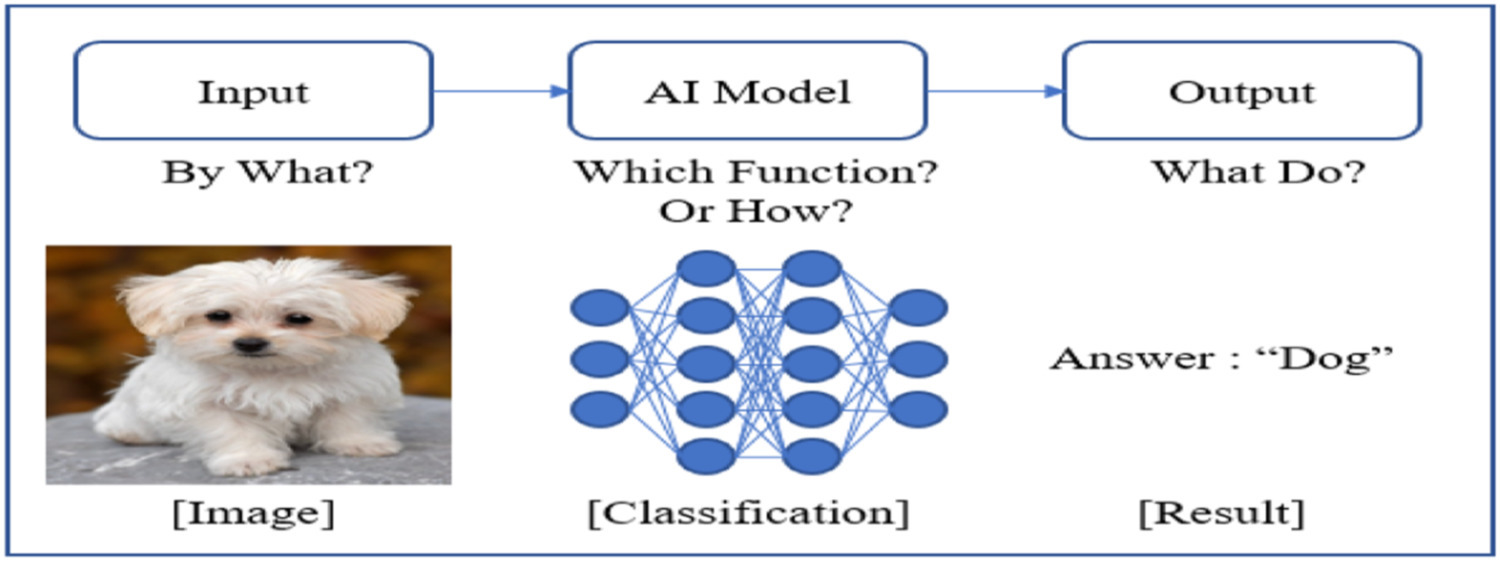
\includegraphics[width=0.5\textwidth]{image/fig 1.png}
                    \caption{مفهوم ساختار IMO}
                    \label{fig:fig_1}
            
                \end{figure}

            \subsubsection{علت استفاده از ساختار IMO}

            ساختار IMO (ورودی-مدل هوش مصنوعی-خروجی) یک چارچوب منطقی و سیستماتیک است که ورودی‌ها و خروجی‌ها را حول مدل هوش مصنوعی متمرکز می‌کند. دلایل استفاده از این ساختار به شرح زیر است:

            \begin{itemize}
                
                \item مرکزیت مدل هوش مصنوعی: ساختار ،IMO مدل هوش مصنوعی را به عنوان هسته اصلی فرآیند تعریف می‌کند. این مدل نتیجه فناوری هوش مصنوعی است که از طریق داده‌ها و الگوریتم‌ها آموزش دیده است. این رویکرد، تمرکز بر مدل هوش مصنوعی را افزایش می‌دهد و باعث می‌شود که تمامی جوانب مرتبط با آن به دقت مورد بررسی قرار گیرند.

                \item یکپارچگی و هماهنگی: حتی در صورت استفاده از چندین مدل هوش مصنوعی در یک سیستم، هر مدل هوش مصنوعی به صورت مستقل و از طریق ساختار IMO خود عمل می‌کند. این ساختار، هماهنگی بین ورودی‌ها و خروجی‌های مختلف مدل‌ها را تضمین می‌کند و از ایجاد تناقضات و مشکلات احتمالی جلوگیری می‌کند.
                
                \item تعریف واضح ورودی‌ها و خروجی‌ها: ورودی‌های مورد نیاز برای عملکرد مدل هوش مصنوعی همان داده‌های مورد نیاز برای یادگیری یا عملکرد مدل هوش مصنوعی هستند. خروجی‌ها نیز نتایج حاصل از فناوری هوش مصنوعی هستند که از طریق داده‌های ورودی تولید می‌شوند. این تعریف واضح، فرآیند شناسایی و مدیریت داده‌ها و نتایج را تسهیل می‌کند.
                
                \item قابلیت استخراج ملاحظات طراحی: تمام ملاحظات طراحی برای پیاده‌سازی عملکرد هوش مصنوعی می‌تواند از طریق ساختار IMO مشتق شود. این شامل انتخاب داده‌های ورودی، طراحی و بهینه‌سازی مدل‌ها، و تحلیل خروجی‌ها است. با استفاده از این ساختار، می‌توان به یک دید جامع و کامل از نیازهای طراحی و پیاده‌سازی مدل‌های هوش مصنوعی دست یافت.

                \item منطق فنی و عملیاتی: از منظر فنی، ساختار IMO به عنوان آغاز و پایان تشکیل فناوری هوش مصنوعی در نظر گرفته می‌شود. این ساختار، فرآیند طراحی و پیاده‌سازی فناوری هوش مصنوعی را به صورت منطقی و سازمان‌یافته هدایت می‌کند. با شناسایی و تحلیل ملاحظات طراحی از طریق ساختار IMO، می‌توان به یک رویکرد منظم و کارآمد در توسعه سیستم‌های هوش مصنوعی دست یافت.

            \end{itemize}

            در نتیجه، استفاده از ساختار IMO به دلیل تمرکز بر مدل هوش مصنوعی، یکپارچگی و هماهنگی بین ورودی‌ها و خروجی‌ها، تعریف واضح نیازمندی‌ها، قابلیت استخراج ملاحظات طراحی، و منطق فنی و عملیاتی، به عنوان یک رویکرد موثر و جامع در طراحی معماری سیستم‌های هوش مصنوعی توصیه می‌شود.

        \subsubsection{ملاحظات فنی برای طراحی معماری سیستم هوش مصنوعی با استفاده از ساختار IMO}

            در این بخش، ملاحظات فنی برای طراحی سیستم‌ها و فناوری هوش مصنوعی با استفاده از ساختار IMO را شرح می‌دهیم. فناوری هوش مصنوعی به طور کلی به دو مرحله تقسیم می‌شود: فرآیند دستیابی به مدل‌های هوش مصنوعی و فرآیند بهره‌برداری از آنها. ساختار IMO در هر دو این مراحل گنجانده شده است، اما تفاوت در محیط است. محیطی که فرآیند دستیابی به مدل‌های هوش مصنوعی در آن انجام می‌شود، عمدتاً یک محیط آزمایشگاهی یا تحقیقاتی است، در حالی که محیطی که مدل هوش مصنوعی در آن اجرا می‌شود، سیستم واقعی است که مدل هوش مصنوعی در آن مستقر شده است. این تفاوت‌های محیطی در نهایت بر داده‌های مورد استفاده برای به دست آوردن مدل هوش مصنوعی و عملکرد مدل هوش مصنوعی به دست آمده تأثیر می‌گذارد. اگر این تفاوت‌ها در طول طراحی معماری نادیده گرفته شوند، مدل هوش مصنوعی ممکن است الزامات عملکرد را در مرحله اکتساب برآورده کند اما در مرحله عملیات واقعی سیستم نتواند آنها را برآورده کند. برای جلوگیری از این امر، در این مطالعه، ساختار IMO را از محیطی که سیستم هوش مصنوعی توسعه‌یافته در آن کار خواهد کرد، شناسایی کرده و از آن برای مشخص کردن الزامات فنی مرتبط با ساختار IMO در فرآیند دستیابی به مدل هوش مصنوعی استفاده می‌کنیم. برای نشان دادن اعتبار رویکردمان، توضیح می‌دهیم که چگونه ساختار IMO از نظر تئوری در هر دو فناوری هوش مصنوعی و دیدگاه‌های سیستم وجود دارد و آنچه باید بر اساس آن طراحی شود.

            \paragraph{3.1.4.1}{دیدگاه فناوری هوش مصنوعی}

                فرآیند دستیابی به فناوری هوش مصنوعی شامل به دست آوردن یک مدل هوش مصنوعی با عملکردهای مورد نظر است. فناوری‌های هوش مصنوعی به طور معمول به یادگیری نظارت شده، یادگیری بدون نظارت و یادگیری تقویتی تقسیم می‌شوند. فرآیند به دست آوردن این فناوری‌های هوش مصنوعی شامل به دست آوردن و عملکرد مدل‌های هوش مصنوعی است. شکل 2 هر فرآیند، روابط آنها و مکان ساختار IMO را نشان می‌دهد.

                \begin{enumerate}
                    
                    \item فرآیند دستیابی به مدل هوش مصنوعی: این فرآیند به طور کلی شامل سه مرحله است: آماده‌سازی آزمایش، طراحی الگوریتم هوش مصنوعی، و آموزش و اعتبارسنجی که معمولاً در یک محیط آزمایشگاهی انجام می‌شود.
                    
                    \begin{itemize}
                        
                        \item آماده‌سازی آزمایش: داده‌های مورد نیاز برای یادگیری نظارت شده/بدون نظارت یا محیطی برای یادگیری تقویتی آماده می‌شود.

                        \item طراحی الگوریتم هوش مصنوعی: ساختار دقیق معماری IMO برای به دست آوردن مدل هوش مصنوعی طراحی می‌شود. ورودی‌ها به شکل شکل یا ابعادی که در الگوریتم هوش مصنوعی استفاده خواهد شد، طراحی می‌شوند.

                        \item آموزش و اعتبارسنجی: وظایف آموزش و اعتبارسنجی تکراری با استفاده از داده‌های (یا محیط) آماده‌شده و الگوریتم هوش مصنوعی انجام می‌شود.
                        
                    \end{itemize}

                    \item فرآیند عملکرد مدل هوش مصنوعی: این فرآیند شامل دو مرحله است: بارگذاری مدل هوش مصنوعی و عملکرد مدل هوش مصنوعی که در یک سیستم در یک محیط عملیاتی واقعی انجام می‌شود.

                    \begin{itemize}
                        
                        \item بارگذاری مدل هوش مصنوعی: وظیفه بارگذاری مدل هوش مصنوعی آموزش‌دیده و الگوریتم‌های آن به حافظه سیستم است.

                        \item عملکرد مدل هوش مصنوعی: سیستم با استفاده از مقادیر ورودی از سیستم و مدل هوش مصنوعی بارگذاری شده، مقادیر خروجی را پیش‌بینی می‌کند.

                    \end{itemize}

                \end{enumerate}

                \begin{figure}[htbp]

                    \centering
                    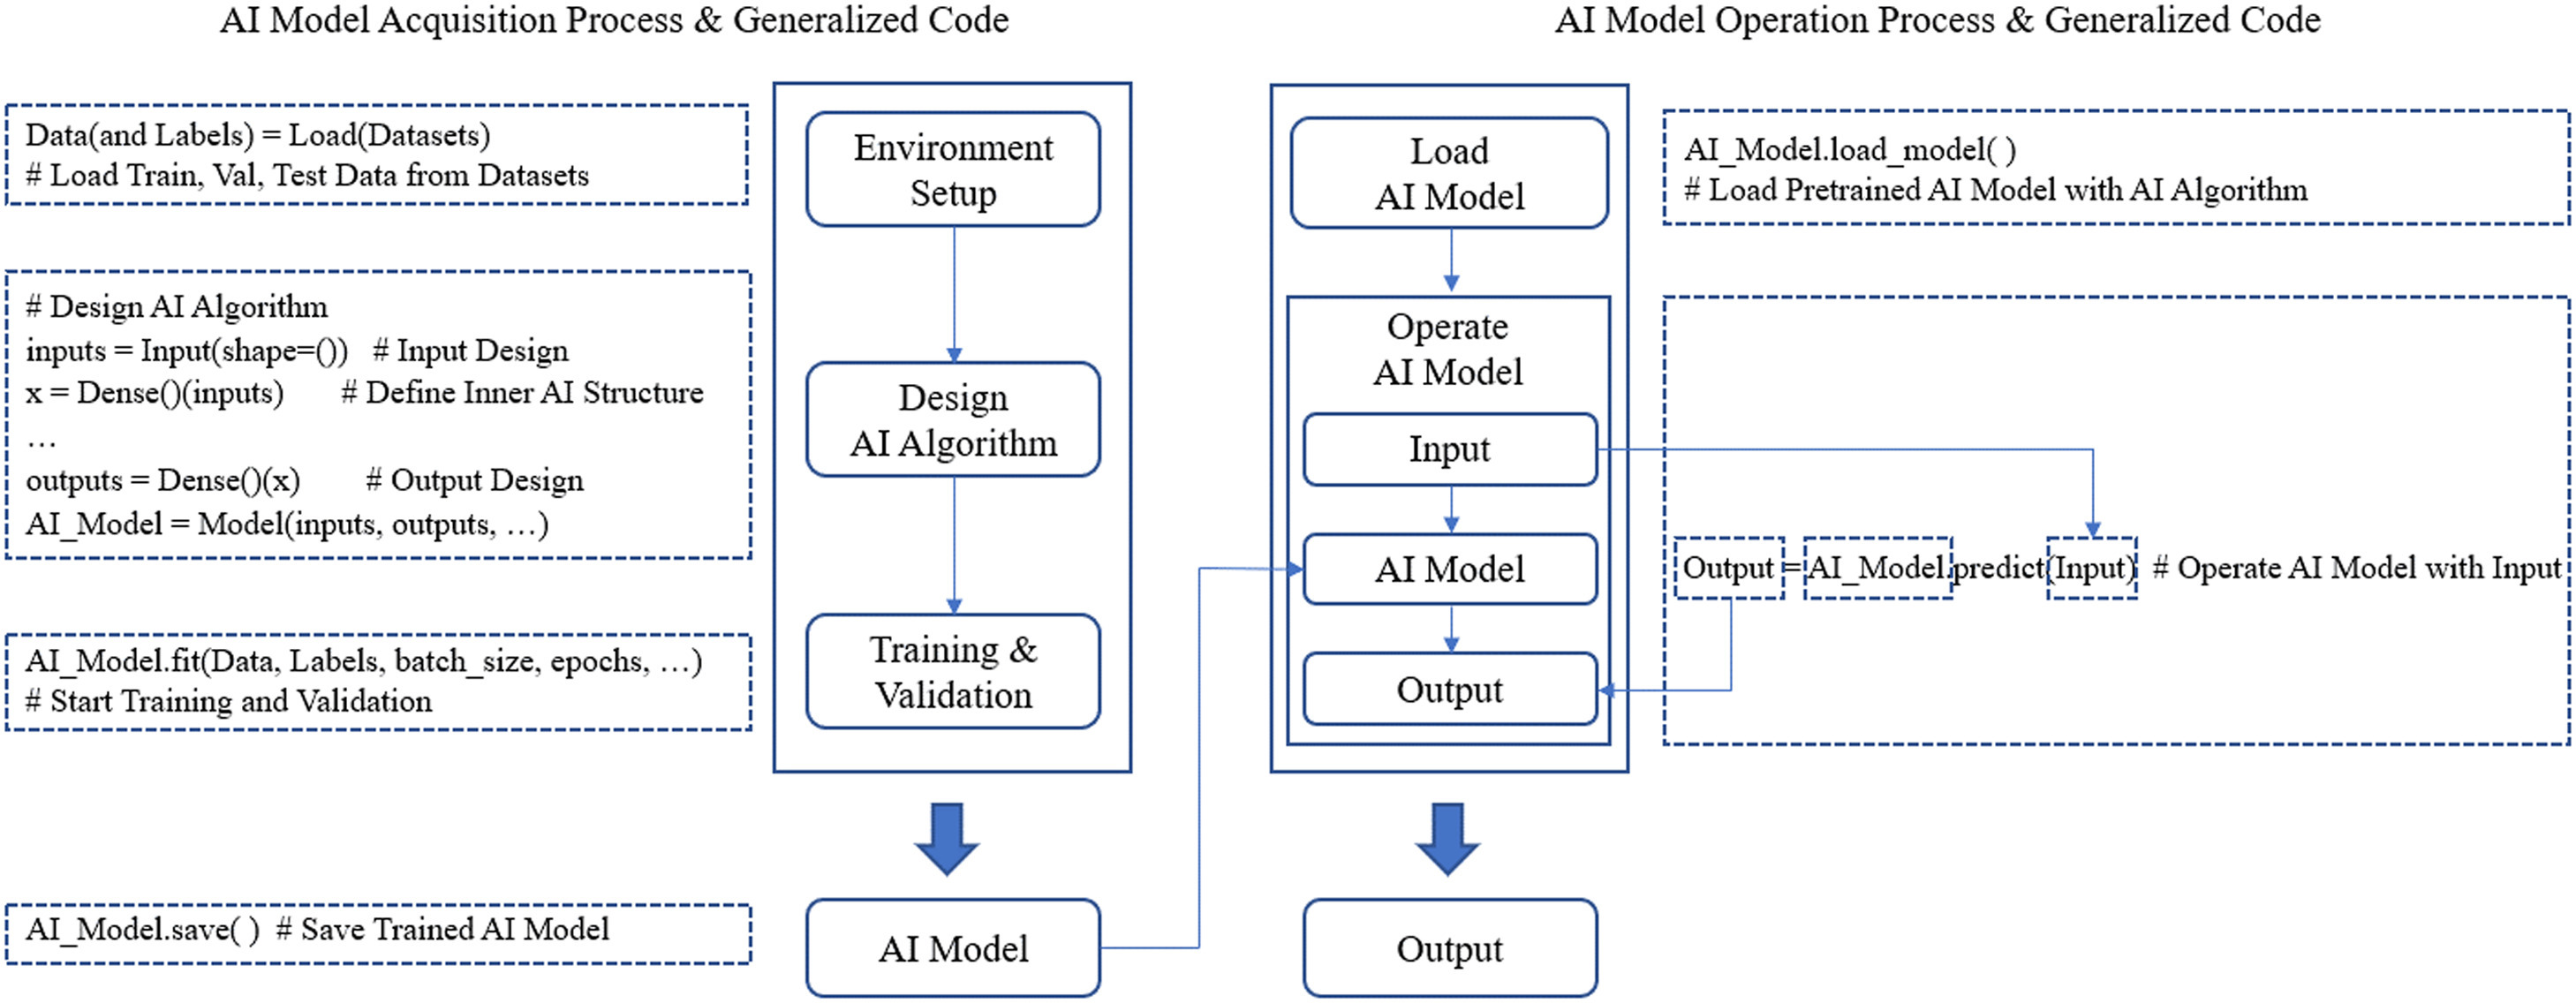
\includegraphics[width=0.8\textwidth]{image/fig 2.png}
                    \caption{فرآیند کسب و عملیات یک مدل هوش مصنوعی و موقعیت ساختار IMO}
                    \label{fig:fig_2}
                
                \end{figure}

            \paragraph{3.1.4.2}{دیدگاه سیستمی}

                سیستم دارای یک معنای گسترده است و می‌تواند به عنوان یک مجموعه متنوع از عناصر مرتبط که با همکاری با یکدیگر برای دستیابی به یک هدف مشترک کار می‌کنند، تعریف شود. بسته به قصد طراح، سیستم از ترکیبی از عناصری که در سطوح مختلف موجود هستند، مانند زیرسیستم‌ها، اجزا و بخش‌ها، از طریق فرآیند تجزیه و تحلیل سیستم تشکیل شده است. فناوری هوش مصنوعی در ماژول نرم‌افزاری که مدل هوش مصنوعی استفاده می‌شود و در سطح اجزای نرم‌افزاری نماینده می‌شود، وجود دارد. به طور خلاصه، از دیدگاه سیستم، یک سیستم هوش مصنوعی می‌تواند به عنوان یک سیستم با یک یا چند مؤلفه هوش مصنوعی تعریف شود، و یک مؤلفه هوش مصنوعی یک مؤلفه سیستم با یک یا چند ساختار IMO است. شکل 3 سلسله مراتب کلی سیستم هوش مصنوعی و چگونگی وجود ساختار IMO را نشان می‌دهد.

                \begin{figure}[htbp]

                    \centering
                    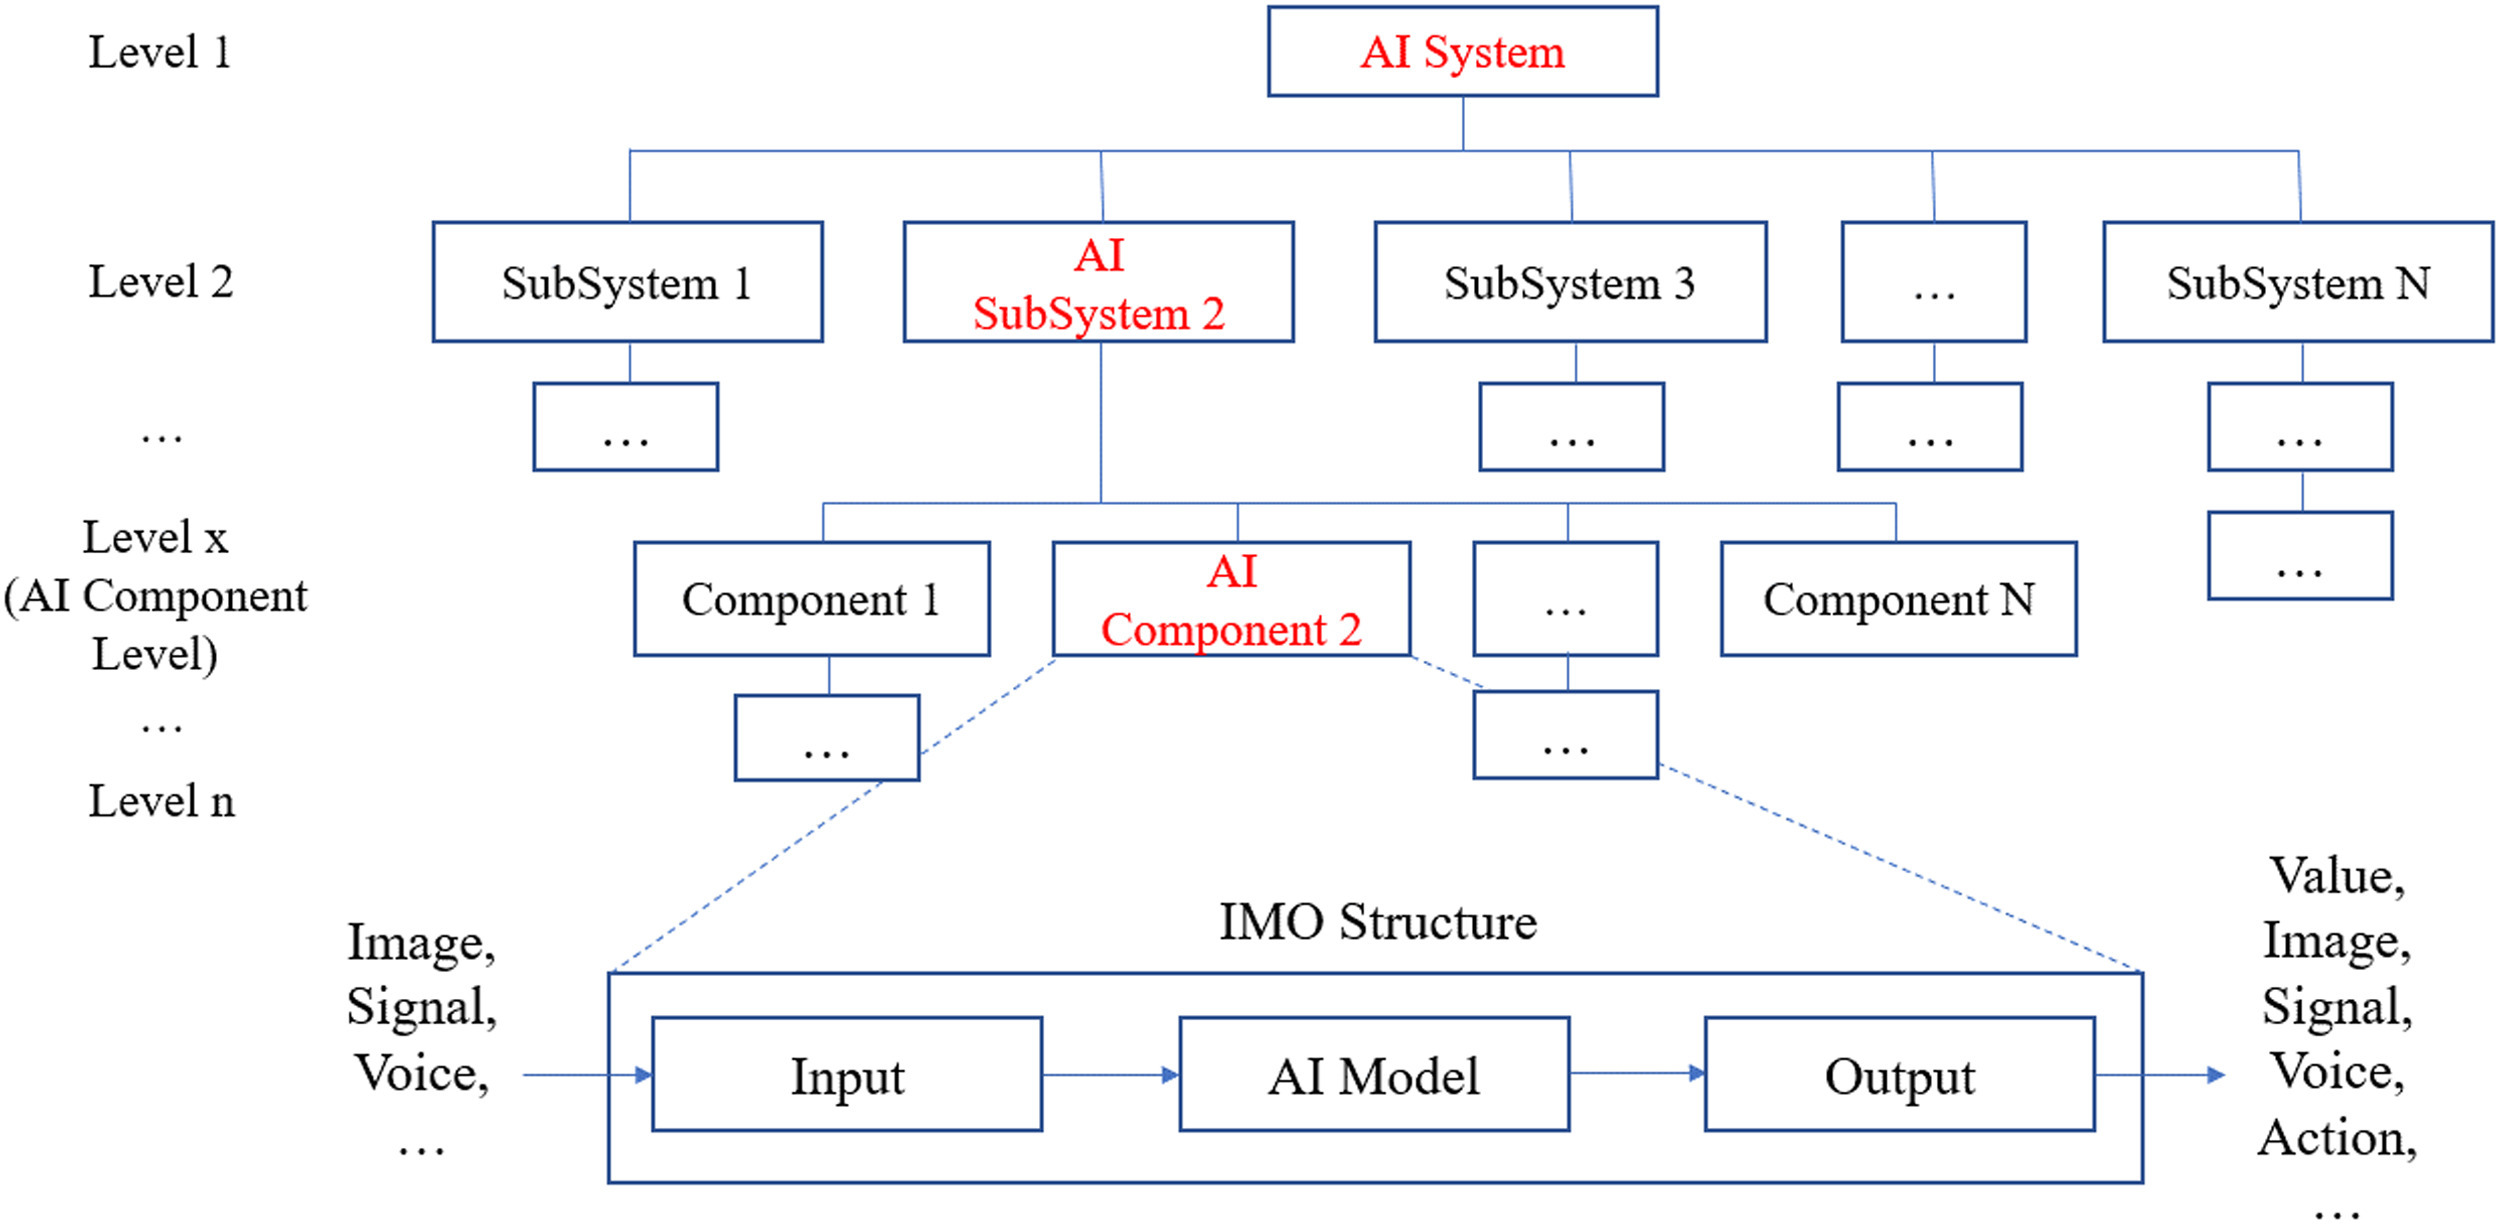
\includegraphics[width=0.6\textwidth]{image/fig 3.png}
                    \caption{سلسله مراتب یک سیستم هوش مصنوعی تعمیم یافته و مکان ساختار IMO}
                    \label{fig:fig_3}
                
                \end{figure}

        \paragraph{3.1.4.3}{ملاحظات فنی برای طراحی معماری سیستم هوش مصنوعی}

            ملاحظات فنی پیشنهاد شده در این مطالعه شامل چهار مورد می‌شود: داده یا محیط، الگوریتم هوش مصنوعی و خروجی، عملکرد هوش مصنوعی و الزامات مؤلفه هوش مصنوعی.

            \begin{enumerate}
                
                \item داده یا محیط: داده و محیط پیش‌نیازهای ضروری برای یادگیری الگوریتم‌های هوش مصنوعی هستند و با قسمت I از ساختار IMO ارتباط دارند. داده تأثیر مستقیمی بر عملکرد مدل‌های هوش مصنوعی دارد. بنابراین، طراحی الزامات روشن برای داده یا محیط هنگام طراحی عملکرد هوش مصنوعی سیستم بسیار حیاتی است. اگر داده یا اطلاعاتی که از محیط عملیاتی واقعی به دست می‌آید با داده یا محیطی که برای به دست آوردن مدل هوش مصنوعی استفاده شده است متفاوت باشد، مدل هوش مصنوعی آموزش دیده شده ممکن است عملکرد ضعیف یا رفتارهای نامطلوبی داشته باشد.

                \item الگوریتم‌های هوش مصنوعی و خروجی: این موارد با مؤلفه‌های M و O از ساختار IMO مرتبط هستند. الگوریتم‌های هوش مصنوعی به الزامات ذینفعان برای کدام عملکرد سیستم هوش مصنوعی باید انجام دهد نقش می‌بینند. خروجی نیز به الزامات ذینفعان برای چگونگی ارائه عملکرد نقش می‌بینند. به عنوان مثال، اگر الزامات ذینفعان برای شناسایی آبجکت‌ها به صورت زمان واقعی از تصاویر باشد، عملکرد هوش مصنوعی شناسایی خواهد بود و خروجی موقعیت شی در تصویر خواهد بود.

                \item عملکرد هوش مصنوعی: به عملکرد یک مدل آموزش دیده هوش مصنوعی اشاره دارد و با عناصر M و O از ساختار IMO ارتباط دارد. روش‌های مختلفی برای اندازه‌گیری عملکرد یک مدل هوش مصنوعی وجود دارد که به نوع و هدف الگوریتم هوش مصنوعی بستگی دارد. بنابراین، الزامات عملکرد هوش مصنوعی باید روش اندازه‌گیری عملکرد مناسبی را انتخاب کنند که در حد امکان نیازهای ذینفعان را برآورده کند.

                \item الزامات مؤلفه‌های هوش مصنوعی: به الزامات سطح سیستم برای عملکرد مدل‌های هوش مصنوعی تهیه شده می‌پردازد، که شامل مؤلفه‌های نرم‌افزاری (SW) مانند سیستم عامل (OS) و مؤلفه‌های سخت‌افزاری (HW) مانند واحد پردازش مرکزی (CPU) و حافظه دسترسی تصادفی (RAM) می‌شود. الزامات مؤلفه‌های هوش مصنوعی با طراحی منابع محاسباتی لازم مرتبط بوده و در نهایت بر روی هزینه تولید سیستم‌های هوش مصنوعی تأثیر می‌گذارد. در فرآیند تهیه مدل هوش مصنوعی، داده‌ها یا محیطی که برای آموزش آماده شده‌اند، به حافظه سیستم بارگذاری شده و وزن‌های مدل هوش مصنوعی به‌طور مکرر محاسبه و به‌روزرسانی می‌شود. در حالی که فرآیند عملکرد مدل هوش مصنوعی تنها نیاز به استنتاج با استفاده از مدل هوش مصنوعی آموزش دیده دارد. بنابراین، هنگام طراحی معماری سیستم، مشخصات سخت‌افزاری مناسب برای عملکرد مدل هوش مصنوعی آموزش دیده باید مدنظر قرار گیرد تا هزینه را در نظر بگیرد، یا تکنولوژی‌های هوش مصنوعی که حتی در محیط‌های با عملکرد پایین هم قابل عملیات هستند، باید مورد بررسی قرار گیرد.

            \end{enumerate}
        
        \subsection{فرآیند طراحی معماری سیستم هوش مصنوعی پیشنهادی}

            در این بخش، فرآیند طراحی معماری سیستم هوش مصنوعی با تمرکز بر روی ساختار IMO شرح داده می‌شود. هدف از این روش، شناسایی و طراحی الزامات فنی برای سیستم‌ها و فناوری‌های هوش مصنوعی است که می‌توانند از فعالیت‌های عملیاتی آینده پشتیبانی کرده و به دستاوردهای سازمان کمک کنند.

            \subsubsection{فرآیند اساسی}

                روش طراحی معماری ارائه شده از سه فعالیت اصلی تشکیل شده است: تعریف مسئله، راه‌حل هوش مصنوعی سیستمی، و راه‌حل فنی هوش مصنوعی. شکل ۴ فرآیند پیشنهادی طراحی معماری سیستم هوش مصنوعی را نشان می‌دهد.

                \begin{itemize}
                    
                    \item تعریف مسئله: هدف این فعالیت، مشخص کردن وضعیت مسئله و جایگزینی است که سازمان می‌خواهد از منظر عملیاتی به آن پرداخته شود. در این مرحله، مسائل سازمان و نقش‌های هوش مصنوعی برای حل مسائل شناسایی می‌شوند.

                    \item راه‌حل هوش مصنوعی سیستمی: هدف این مرحله، طراحی ساختاری است که بتواند الزامات سازمان را که از منظر عملیاتی شناسایی شده‌اند، از دیدگاه سیستمی به تجسم درآورد. در این مرحله، ساختار سیستم و الزامات عنصر هوش مصنوعی که می‌توانند نقش‌های هوش مصنوعی شناسایی شده را انجام دهند، مشخص می‌شوند.

                    \item راه‌حل فنی هوش مصنوعی: هدف این مرحله، تشخیص الزامات فنی برای به دست آوردن فناوری هوش مصنوعی است که می‌تواند نقش‌های هوش مصنوعی شناسایی شده را انجام دهد. در این مرحله، داده‌ها و عملکردهای هوش مصنوعی مورد نیاز برای توسعه مدل‌های هوش مصنوعی که در سیستم واقعی استفاده خواهند شد، مشخص می‌شوند.

                \end{itemize}

                فرآیند طراحی معماری با استفاده از فعالیت‌های مهندسی سیستم معمولاً بر روی راه‌حل‌های سیستم تمرکز دارد. با استفاده از در نظر گرفتن الزامات فنی مشتق شده از ساختار IMO، فناوری‌های هوش مصنوعی مشخص می‌شوند. سه فعالیت تا زمان کامل شدن طراحی معماری تکرار می‌شوند که منجر به طراحی نهایی معماری سیستم هوش مصنوعی می‌شود.

                \begin{figure}[htbp]

                    \centering
                    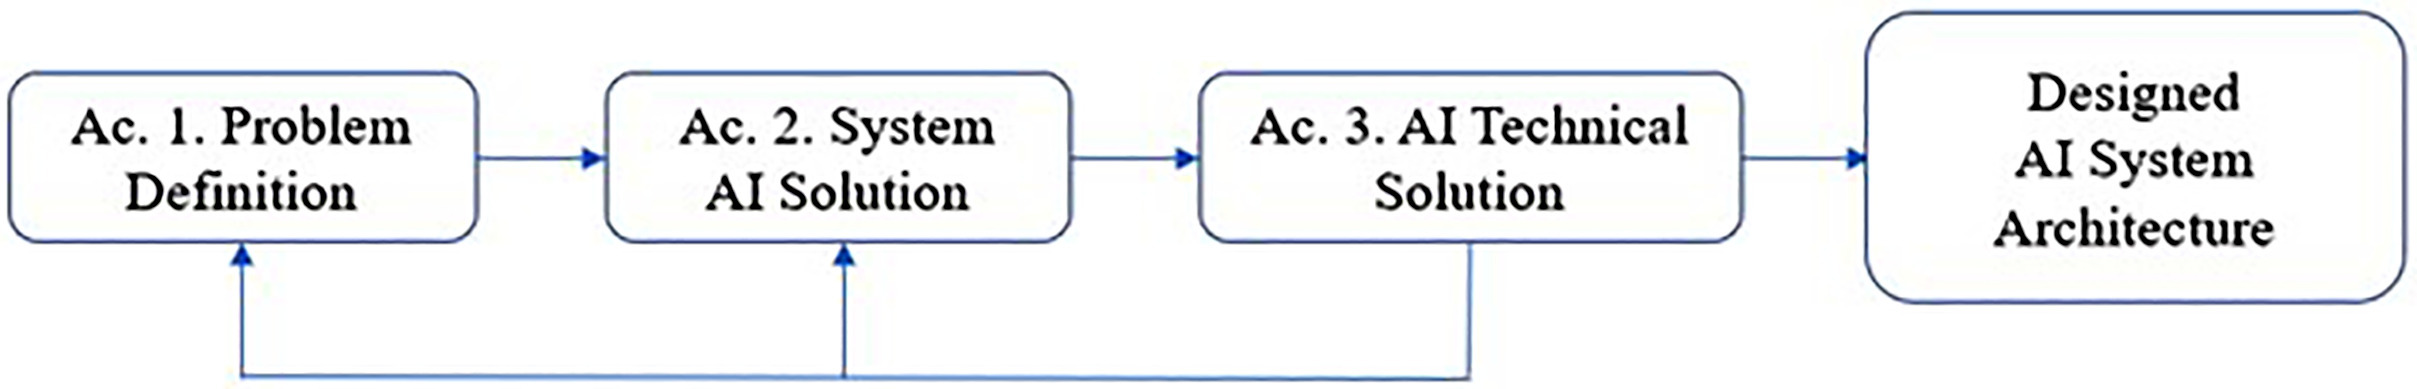
\includegraphics[width=0.6\textwidth]{image/fig 4.png}
                    \caption{فرآیند اساسی روش طراحی معماری سیستم هوش مصنوعی پیشنهادی}
                    \label{fig:fig_4}
                
                \end{figure}

            \subsubsection{فرآیند دقیق}

                جزئیات فرآیند پیشنهادی به شرح زیر است:

                \begin{figure}[htbp]

                    \centering
                    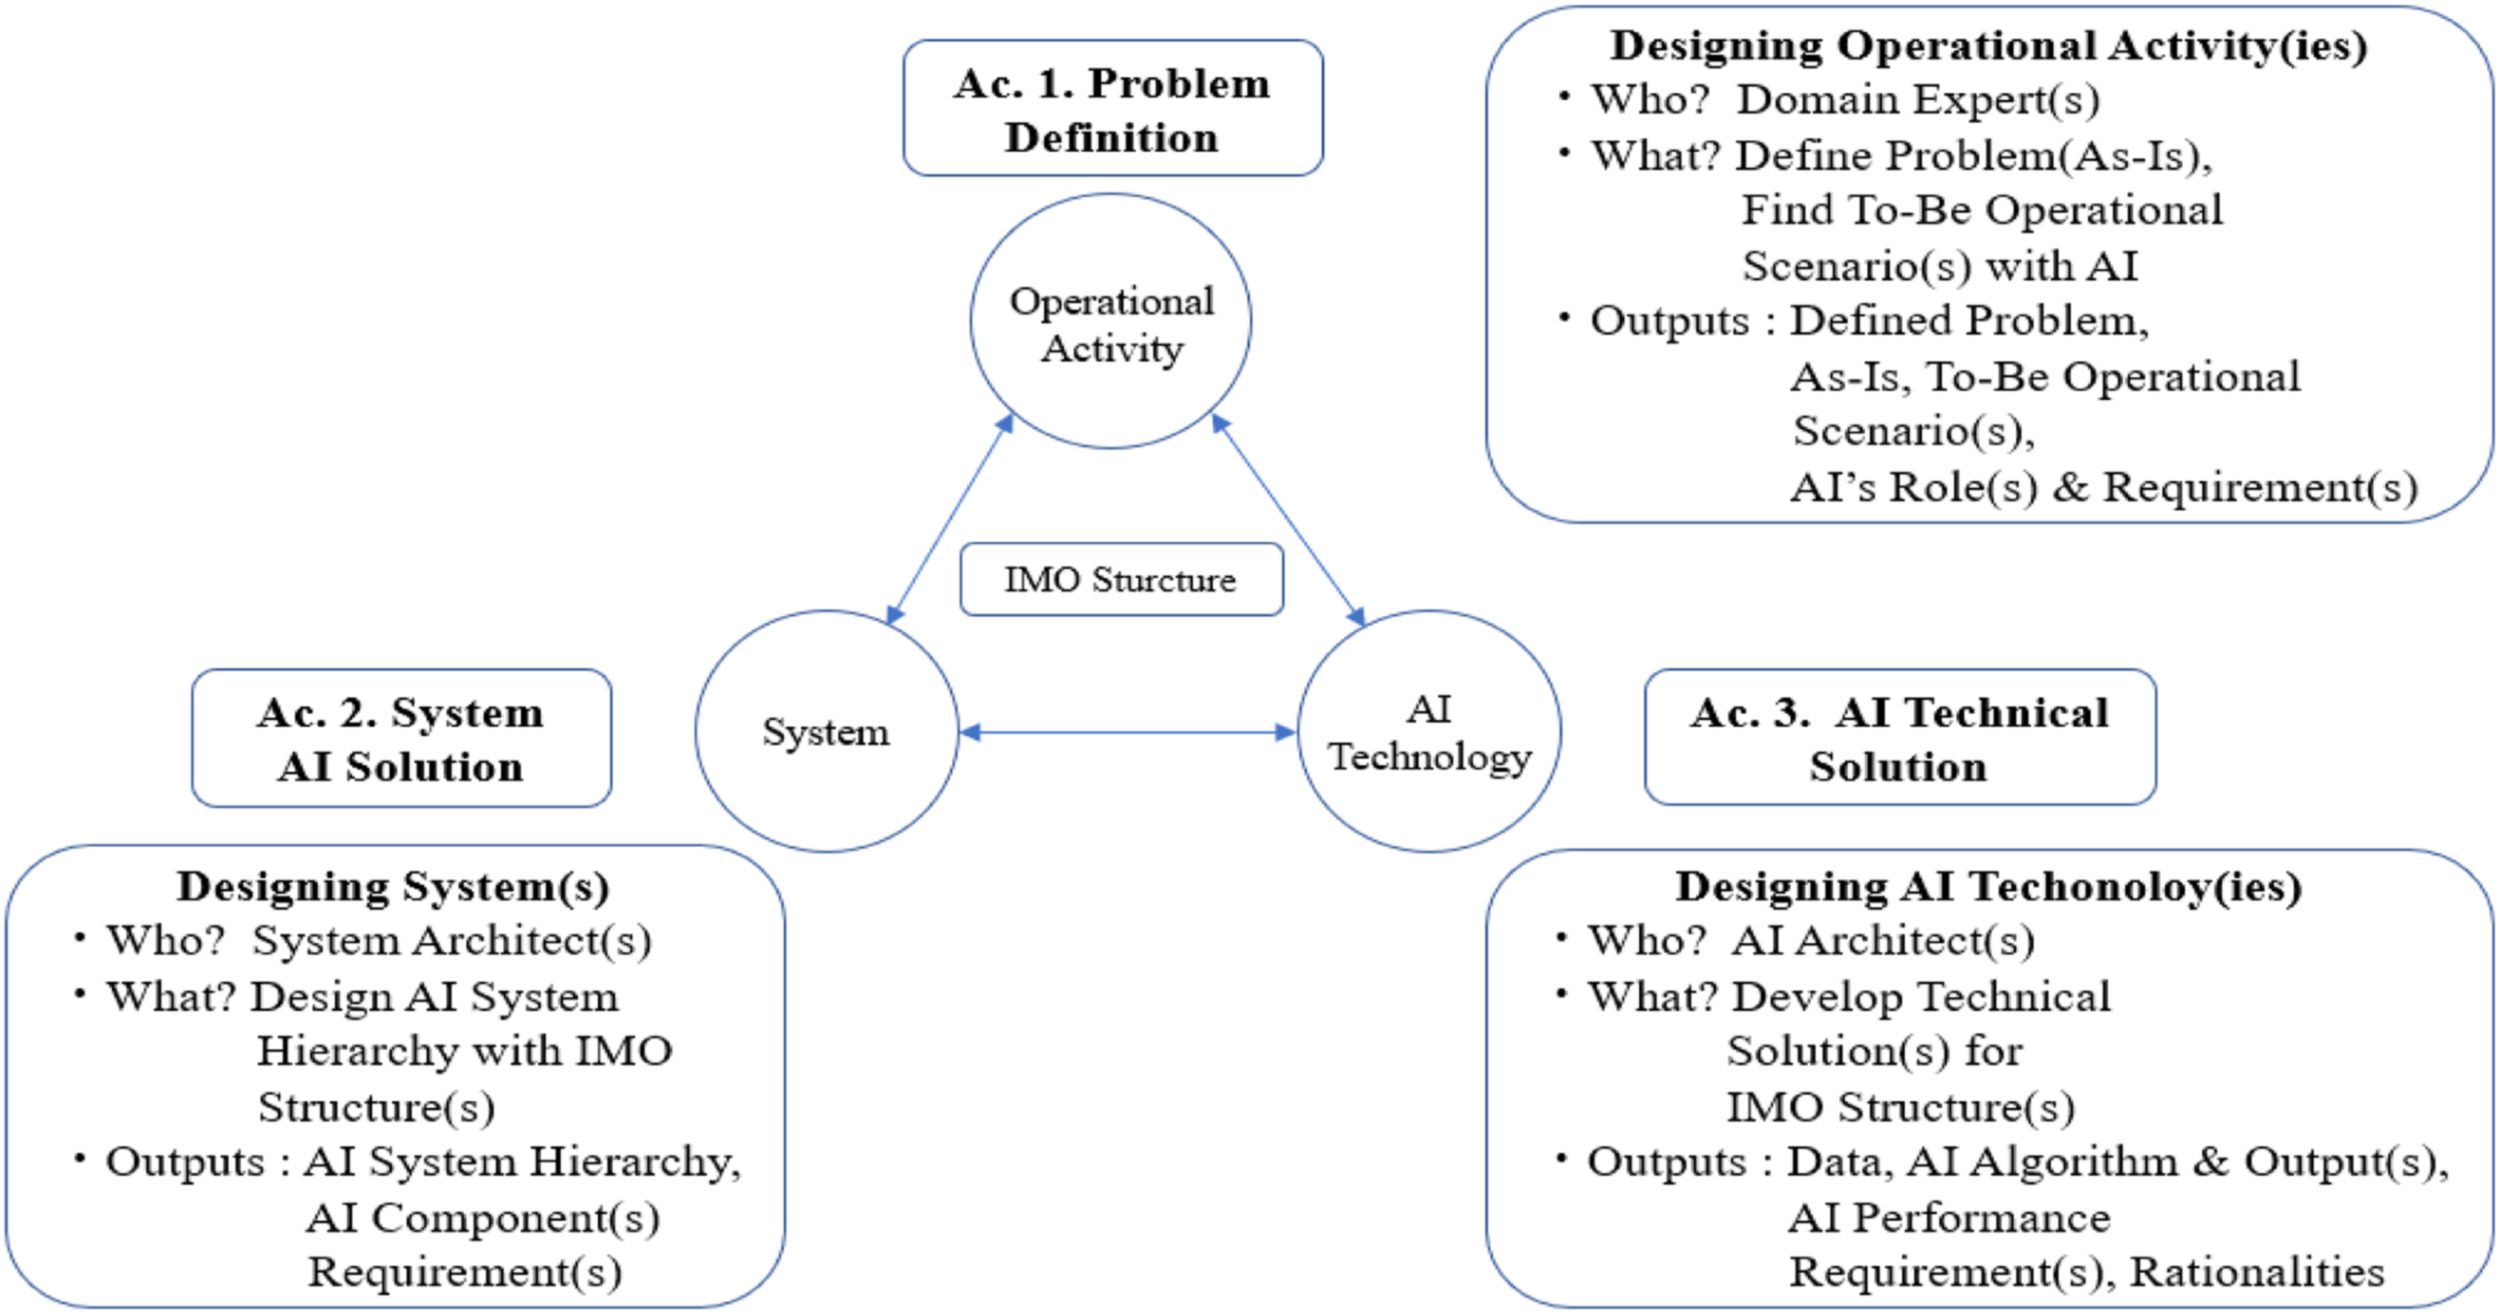
\includegraphics[width=0.8\textwidth]{image/fig 5.png}
                    \caption{رابطه متقابل بین سه فعالیت طراحی پیشنهادی}
                    \label{fig:fig_5}
                
                \end{figure}

                \begin{itemize}
                    
                    \item مرحله تعریف مسئله: مسائل حوزه تخصصی سازمان از طریق فعالیت‌های عملیاتی تعریف می‌شوند و نقش هوش مصنوعی بر اساس آن‌ها مشخص می‌شود. این مرحله اصولاً توسط کارشناسان حوزه انجام می‌شود. فعالیت‌های جزئی این مرحله شامل چهار فعالیت است:
                    
                    \begin{itemize}
                        
                        \item شناسایی مسائل کلیدی سازمان.

                        \item تعیین نقش‌های هوش مصنوعی در حل مسائل.

                        \item تحلیل فرآیندهای عملیاتی موجود.

                        \item شناسایی معیارهای عملکردی مورد انتظار.

                    \end{itemize}

                    \begin{figure}[htbp]

                        \centering
                        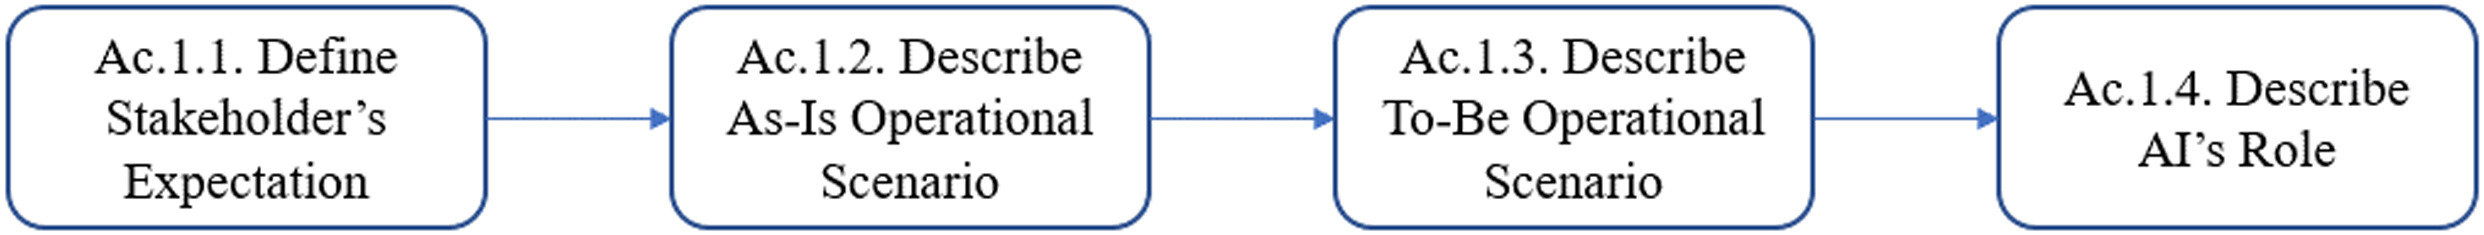
\includegraphics[width=0.8\textwidth]{image/fig 6.png}
                        \caption{رابطه متقابل بین سه فعالیت طراحی پیشنهادی}
                        \label{fig:fig_6}
                    
                    \end{figure}

                    خروجی‌های اصلی این مرحله شامل تعریف مسائل، نقش‌های هوش مصنوعی، تحلیل فرآیندهای عملیاتی و معیارهای عملکردی است.

                    \begin{table}[htbp]
                        
                        \centering
                        \caption{خروجی‌های اصلی مرحله تعریف مسئله}
                        \begin{tabularx}{\textwidth}{X}
                        
                            \specialrule{1pt}{1pt}{5pt}
                            \multicolumn{1}{c}{انتظارات ذینفعان [Ac.1.1.]} \\
                            \specialrule{0.5pt}{1pt}{1pt}
                            
                            شرح: مسئله‌هایی که باید با استفاده از هوش مصنوعی حل شوند را توصیف کنید یا تعریف کنید. \\
                            
                            \specialrule{0.5pt}{1pt}{5pt}
                            \multicolumn{1}{c}{سناریو(های) as-is [Ac.2.1.]} \\
                            \specialrule{0.5pt}{1pt}{1pt}
                            
                            شرح: مسائل فعلی که باید با استفاده از هوش مصنوعی حل شوند را به عنوان یک یا چند سناریو عملی از طریق روش‌های مناسب مانند EFFBD(s) و متن‌ها بیان کنید. \\
                            شرایط: عواملی که بر سناریو(های) عملی تأثیر می‌گذارند مانند زمان، فضا و سایر موارد را شرح دهید. \\
                            
                            \specialrule{0.5pt}{1pt}{5pt}
                            \multicolumn{1}{c}{سناریو(های) to-be [Ac.3.1.]} \\
                            \specialrule{0.5pt}{1pt}{1pt}
                            
                            شرح: بیان کنید سناریو(های) عملی آینده که مسئله(ها) با استفاده از هوش مصنوعی حل می‌شود(ند)، از طریق روش‌های مناسب مانند EFFBD(s) و متن. \\
                            شرایط: عواملی که بر سناریو(های) عملی تأثیر می‌گذارند، مانند زمان، فضا و سایر موارد را شرح دهید. \\
                            
                            \specialrule{0.5pt}{1pt}{5pt}
                            \multicolumn{1}{c}{نقش(های) هوش مصنوعی} \\
                            \specialrule{0.5pt}{1pt}{1pt}
                            
                            شرح: نقش(های) و اجرا کننده(ها) های هوش مصنوعی مورد نیاز برای سناریو(های) عملی آینده را (با در نظر گرفتن عنصر M و عنصر O از ساختار IMO) بیان کنید. \\
                            
                            \specialrule{1pt}{1pt}{1pt}
                            
                        \end{tabularx}
                    \end{table}

                    \item مرحله راه حل هوش مصنوعی سیستمی: سناریوی عملیاتی طراحی شده از منظر اجراکنندگان در مرحله تعریف مسئله به یک منظر سیستم تبدیل می‌شود. این مرحله اصولاً توسط کارشناسان سیستم انجام می‌شود. فعالیت‌های جزئی این مرحله شامل چهار فعالیت است:
                    
                    \begin{itemize}
                        
                        \item طراحی ساختار کلی سیستم.

                        \item شناسایی اجزای سیستم.

                        \item تعیین الزامات عملکردی اجزای سیستم.

                        \item ارزیابی ارتباطات و تعاملات بین اجزای سیستم.

                    \end{itemize}

                    \begin{figure}[htbp]

                        \centering
                        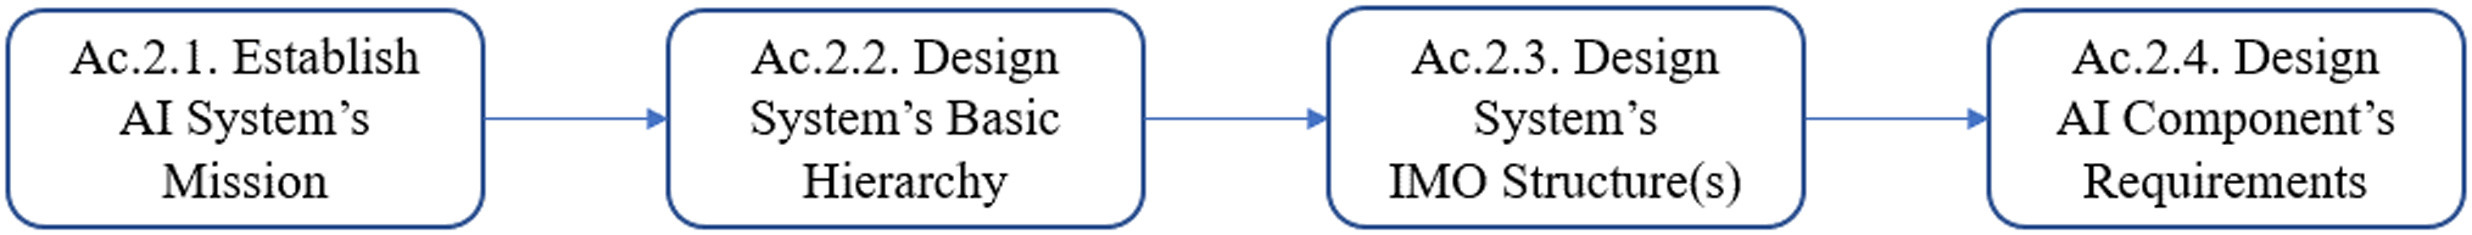
\includegraphics[width=0.8\textwidth]{image/fig 7.png}
                        \caption{چهار فعالیت در مرحله راه حل هوش مصنوعی سیستم}
                        \label{fig:fig_7}
                    
                    \end{figure}

                    \begin{table}[htbp]
                        
                        \centering
                        \caption{خروجی‌های اصلی مرحله راه حل هوش مصنوعی سیستم}
                        \begin{tabularx}{\textwidth}{X}
                        
                            \specialrule{1pt}{1pt}{5pt}
                            \multicolumn{1}{c}{ماموریت سیستم هوش مصنوعی [Ac.1.2.]} \\
                            \specialrule{0.5pt}{1pt}{1pt}
                            
                            توضیحات: ماموریت سیستم هوش مصنوعی را بیان کنید \\

                            \specialrule{1pt}{1pt}{5pt}
                            \multicolumn{1}{c}{راه حل سیستم هوش مصنوعی} \\
                            \specialrule{0.5pt}{1pt}{1pt}

                            توضیحات: سلسله مراتب سیستم هوش مصنوعی و ساختار IMO را بیان کنید. (در زیر یک مثال آورده شده است) \\
                            
                            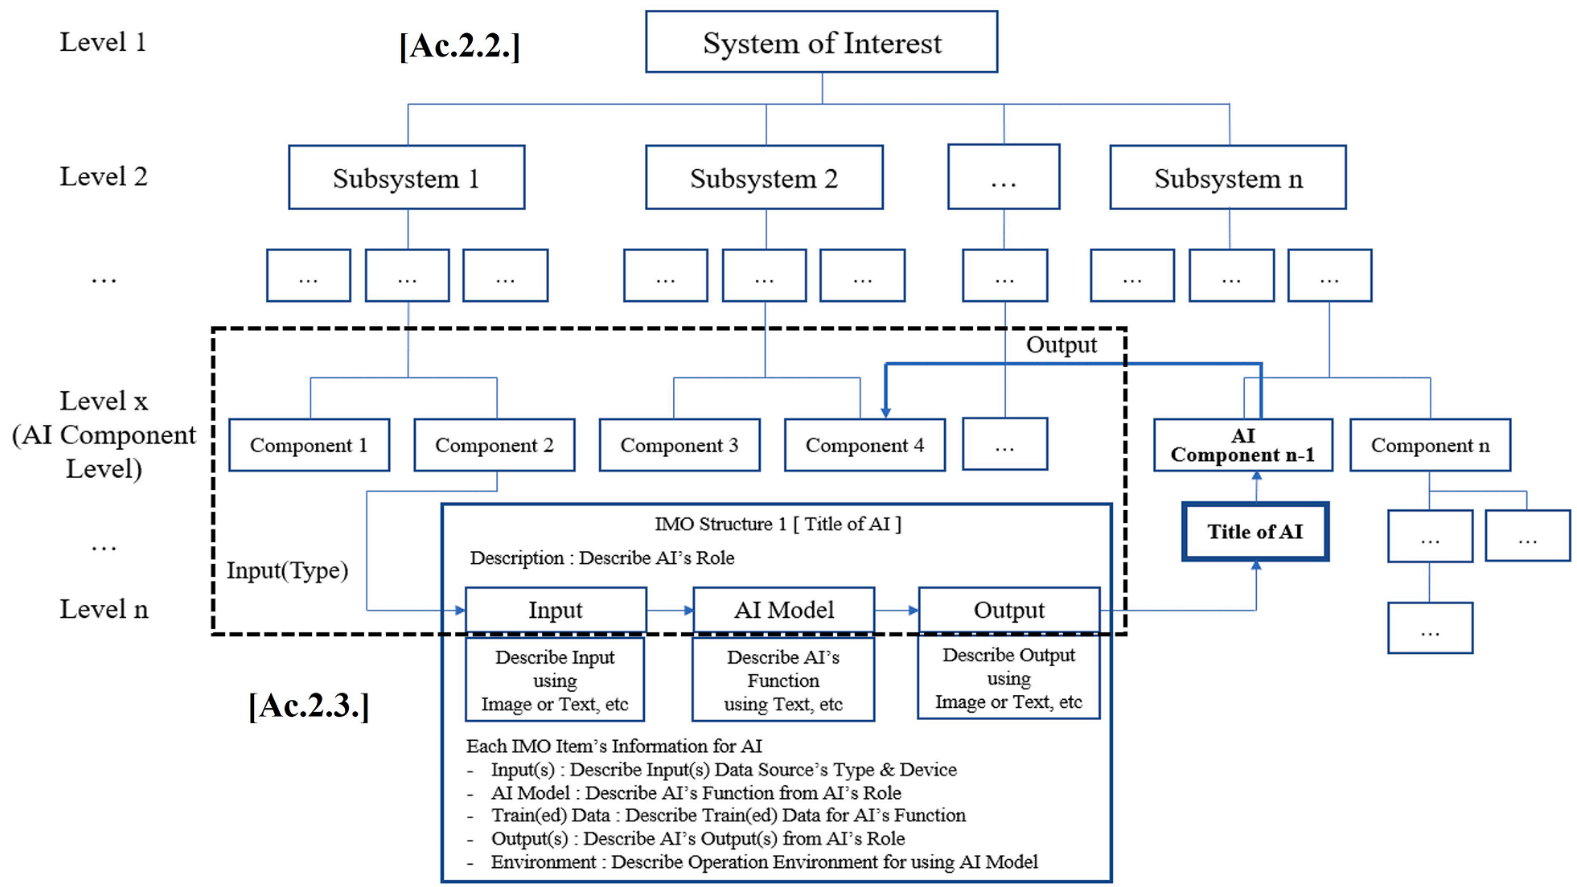
\includegraphics[width=1\linewidth]{image/fig table 2.png} \\

                            \specialrule{0.5pt}{1pt}{5pt}
                            \multicolumn{1}{c}{مولفه(های) هوش مصنوعی مورد نیاز(ها) [Ac.4.2.]} \\
                            \specialrule{0.5pt}{1pt}{1pt}
                            
                            توضیحات: نیاز(های) سطح سیستم را برای اجرای مدل هوش مصنوعی شرح دهید. \\
                            
                            \specialrule{1pt}{1pt}{1pt}
                            
                        \end{tabularx}
                        
                    \end{table}

                    \begin{table}[htbp]

                        \centering
                        \caption{خروجی اصلی در مرحله راه حل فنی هوش مصنوعی}
                        \begin{tabularx}{\textwidth}{c c c c X}

                            \vspace{-10pt}\\

                            \hline

                            \multicolumn{5}{c}{نقش هوش مصنوعی [Ac.4.3.]}\\
                            
                            \hline

                            \multicolumn{5}{c}{راه حل داده}\\

                            \multicolumn{1}{c}{I} & \multicolumn{1}{r}{ورودی} & \multicolumn{1}{r}{نوع} &  & نوع اقلام منبع ورودی را شرح دهید. (به طور مثال: تصویر، سیگنال) \\
                            & \multicolumn{1}{r}{منبع} & \multicolumn{1}{r}{صفت} &  & اطلاعات دقیقی که منبع ورودی را نشان می دهد را شرح دهید. (به عنوان مثال: وضوح، نرخ تجدید، \dots) \\
                            & \multicolumn{1}{r}{داده/محیط} & \multicolumn{1}{r}{صفت} & \multicolumn{1}{r}{نوع، میزان} & نوع و مقدار داده (یا محیط) مورد نیاز را شرح دهید. \\
                            & \multicolumn{1}{r}{نیازمندی‌ها} &  & \multicolumn{1}{r}{شرایط تفصیلی} & شرایط مورد نیازی که باید در داده ها (یا محیط) گنجانده شود را شرح دهید. (به عنوان مثال: عوامل محیطی شناسایی شده در (OV \\
                            & \multicolumn{1}{r}{بنیاد و پایه} & \multicolumn{1}{r}{منبع ورودی} &  & دلیل انتخاب عنصر I را شرح دهید. \\
                            &  & \multicolumn{2}{r}{نیازمندی‌های داده/محیط} & دلیل انتخاب الزامات عنصر I را شرح دهید. \\

                            \multicolumn{5}{c}{راه حل تکنیک هوش مصنوعی}\\

                            \multicolumn{1}{c}{M} & \multicolumn{1}{r}{مدل هوش مصنوعی} & \multicolumn{2}{c}{نوع} & انواع الگوریتم های هوش مصنوعی را توضیح دهید. (به عنوان مثال: طبقه بندی، پیش بینی) \\
                            &  & \multicolumn{2}{c}{الگوریتم} & عنوانی را که نشان دهنده الگوریتم هوش مصنوعی است توضیح دهید. \\
                            &  & \multicolumn{1}{r}{محیط} & \multicolumn{1}{r}{DEV} & محیط توسعه برای دستیابی به مدل هوش مصنوعی را شرح دهید. \\
                            &  &  & \multicolumn{1}{r}{OPS} & محیط مورد نیاز برای اجرای مدل هوش مصنوعی بدست آمده را شرح دهید. \\
                            & \multicolumn{1}{r}{بنیاد و پایه} & \multicolumn{3}{r}{دلیل انتخاب عنصر M را شرح دهید.} \\

                            \multicolumn{1}{c}{O} & \multicolumn{1}{r}{خروجی} & \multicolumn{3}{r}{شکل یا محتوای مقادیر خروجی مدل هوش مصنوعی را شرح دهید.} \\
                            & \multicolumn{1}{r}{عملکرد هوش مصنوعی} & \multicolumn{3}{r}{الزامات عملکرد مدل هوش مصنوعی را با اندازه‌گیری‌ها (یا معیارهای) مناسب توصیف کنید.} \\
                            & \multicolumn{1}{r}{نیازمندی‌ها} &  &  &  \\
                            & \multicolumn{1}{r}{بنیاد و پایه} & \multicolumn{1}{r}{خروجی} &  & \multicolumn{1}{r}{دلیل انتخاب خروجی را شرح دهید.} \\
                            &  & \multicolumn{2}{r}{عملکرد هوش مصنوعی} & \multicolumn{1}{r}{دلیل انتخاب عملکرد هوش مصنوعی را شرح دهید.} \\
                            
                            \multicolumn{2}{c}{دلیل نقش هوش مصنوعی} & \multicolumn{3}{r}{\multirow{2}{*}{توضیح دهید که چگونه ساختار کاملاً طراحی شده IMO در نهایت به نقش هوش مصنوعی دست می یابد.}} \\
                            \multicolumn{2}{c}{در سیستم مورد علاقه} & \\

                            \hline

                        \end{tabularx}
                        
                    \end{table}

                    خروجی‌های اصلی این مرحله شامل طراحی ساختار سیستم، شناسایی اجزای سیستم و تعیین الزامات عملکردی است.

                    \item مرحله راه حل فنی هوش مصنوعی: موارد فنی هوش مصنوعی برای اجرای نقش‌های شناسایی شده طراحی یا شناسایی می‌شوند. این مرحله با همکاری کارشناسان هوش مصنوعی و همچنین کارشناسان حوزه و سیستم انجام می‌شود. فعالیت‌های جزئی این مرحله شامل چهار فعالیت است:

                    \begin{itemize}
                        
                        \item تحلیل داده‌های مورد نیاز برای توسعه مدل‌های هوش مصنوعی.

                        \item طراحی و انتخاب الگوریتم‌های هوش مصنوعی.

                        \item ارزیابی و تست عملکرد مدل‌های هوش مصنوعی.

                        \item تعیین الزامات منابع محاسباتی و سخت‌افزاری.

                    \end{itemize}

                    \begin{figure}[htbp]

                        \centering
                        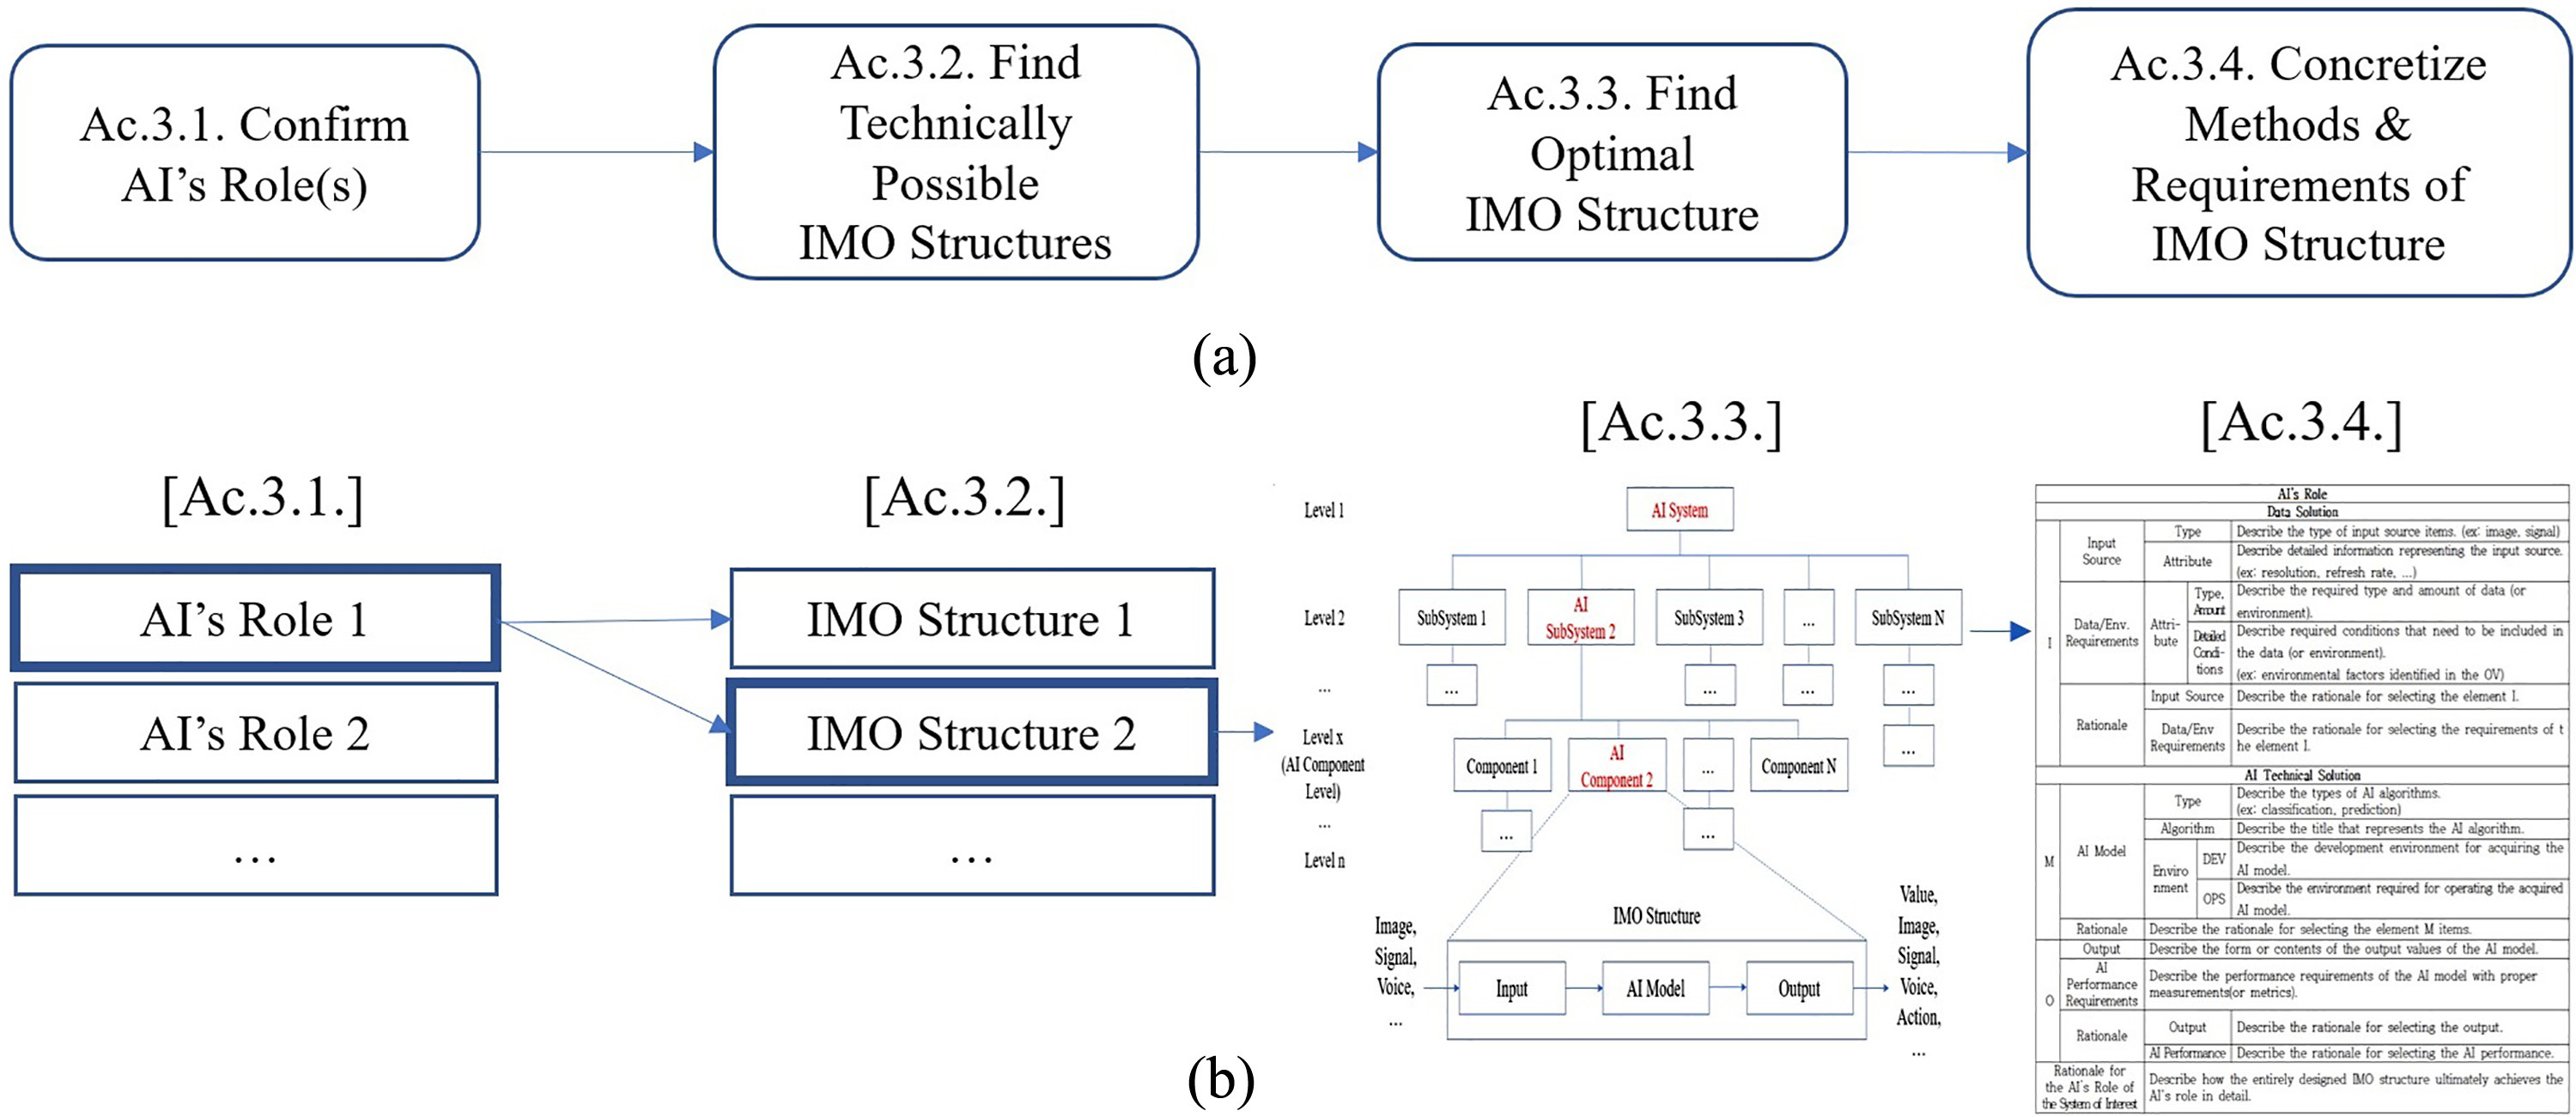
\includegraphics[width=0.8\textwidth]{image/fig 8.png}
                        \caption{الف) چهار فعالیت در مرحله حل فنی هوش مصنوعی ب) شرح گرافیکی مرحله راه حل فنی هوش مصنوعی.}
                        \label{fig:fig_8}
                    
                    \end{figure}

                    خروجی‌های اصلی این مرحله شامل تحلیل داده‌ها، طراحی الگوریتم‌های هوش مصنوعی، ارزیابی عملکرد مدل‌ها و تعیین الزامات منابع محاسباتی است.

                \end{itemize}

                فرآیند طراحی معماری، با تمرکز بر ساختار ،IMO یک رویکرد جامع و مکرر برای شناسایی و طراحی الزامات فنی سیستم‌های هوش مصنوعی فراهم می‌کند که می‌تواند به دستاوردهای سازمان کمک کند.

    \section{نمونه موردی و تحلیل اثربخشی}

        در این مطالعه، یک روش‌شناسی برای طراحی معماری سیستم‌های هوش مصنوعی که سازمان‌ها به آن‌ها نیاز دارند، از طریق ساختار IMO شرح داده شده است. روش‌شناسی ارائه شده در این مقاله سیستم‌های هوش مصنوعی و فناوری‌های هوش مصنوعی مورد نیاز را بر اساس فعالیت‌های عملیاتی آینده که توسط سازمان تصور می‌شود، طراحی می‌کند. علاوه بر این، مفهوم ساختار IMO معرفی شده است تا نیازمندی‌های فنی برای توسعه مدل‌های هوش مصنوعی مورد نیاز را شناسایی کند. به عبارت دیگر، روش‌شناسی ارائه شده محدودیت‌های مطالعات موجود که فقط نیازمندی‌های سطح انتزاعی را شناسایی می‌کنند، برطرف می‌کند و می‌تواند طراحی را با نیازمندی‌های خاص برای توسعه مدل‌های هوش مصنوعی به صورت عملی مشخص کند. در این بخش، با استفاده از روش‌شناسی پیشنهادی، مطالعات موردی را توضیح داده و کارایی آن را ارزیابی می‌کنیم.

        \subsection{مورد نمونه}

            به عنوان یک نمونه از روش پیشنهادی، مثالی از یک سیستم ایمنی خودران برای یک وسیله نقلیه مجهز به دو وظیفه هوش مصنوعی ارائه می‌دهیم: جلوگیری از خواب آلودگی راننده و رانندگی خودکار. نتایج نمایش داده شده از طریق خروجی‌های اصلی سه مرحله از روش پیشنهادی است: تعریف مسئله (ارجاع داده شود به جدول 4)، راه‌حل سیستم هوش مصنوعی (ارجاع داده شود به جدول 5) و راه‌حل فنی هوش مصنوعی (ارجاع داده شود به جدول‌های 6 و 7).

        \subsection{تحلیل اثربخشی روش پیشنهادی}

            روش پیشنهادی یک روش‌شناسی برای انجام طراحی معماری سیستم در سطح مفهومی است تا هوش مصنوعی را با موفقیت در سازمان‌ها پیاده‌سازی کند. بنابراین، انجام مقایسه عینی از اثربخشی آن آسان نیست. برای غلبه بر این مشکل، اثربخشی روش‌شناسی از طریق تحلیل‌های منطقی از سه منظر ارائه می‌شود. اولاً، بهبودهای جزئیات روش‌شناسی در مقایسه با مطالعات قبلی ارائه شده است. ثانیاً، نشان داده می‌شود که چگونه پژوهش می‌تواند به پیشرفت علمی در مقایسه با مطالعات در حوزه تحقیقاتی مشابه طراحی معماری سیستم کمک کند. ثالثاً، نشان داده می‌شود که روش‌شناسی چقدر می‌تواند احتمال موفقیت در پیاده‌سازی هوش مصنوعی در سازمان‌ها را که هدف نهایی این مطالعه است، بهبود بخشد. در نهایت، برای ارائه عینی‌تر اثربخشی روش‌شناسی، نتایج تحلیل و ارزیابی گروهی از کارشناسان به صورت شفاف ارائه می‌شود. این گروه کارشناسی شامل پنج برنامه‌ریز و توسعه‌دهنده هوش مصنوعی بود.

        \subsection{تحلیل مقایسه کیفی با تحقیقات موجود}

            در این بخش، به ارائه‌ سهم نظری روش‌شناسی از طریق مقایسه‌ی کیفی موارد و نتایج تحقیقاتی موجود که برای پیاده‌سازی موفق هوش مصنوعی انجام شده‌اند، پرداخته شده است. برای تحلیل مقایسه‌ی منطقی نتایج تحقیقات، از چهار سوال Q1) تا (Q4 که در مقدمه به عنوان اهداف تحقیقاتی ارائه شده‌اند، به عنوان معیارهای ارزیابی استفاده شده است. این سوالات نمی‌توانند به عنوان تمامی شرایط برای پیاده‌سازی موفق هوش مصنوعی در نظر گرفته شوند، زیرا طراحی سیستم‌های هوش مصنوعی برای پیاده‌سازی موفق هوش مصنوعی نیازمند نه تنها نیازهای فنی بلکه نیازهای غیرفنی مانند شفافیت، اعتمادپذیری و انصاف نیز می‌باشد. بنابراین، چهار معیار ارزیابی برای ارزیابی و تحلیل منصفانه در چارچوب هدف و دامنه این مطالعه استفاده شده‌اند. جدول 8 زیر هر سوال و هدف آن و نتایج مقایسه منطقی بین تحقیقات موجود و روش‌شناسی ما را نشان می‌دهد.

            همان‌طور که شرح داده شده است، تحقیقات موجود در مورد پیاده‌سازی موفق هوش مصنوعی در سازمان‌ها از دیدگاه‌های مختلف علمی مانند قابلیت‌های سازمانی، فرآیندهای مهندسی سیستم، مهندسی نیازمندی‌ها و طراحی معماری انجام شده است. جزئیات تحقیقات موجود شرح داده شده و در اینجا حذف شده است. از طریق تلاش‌های بسیاری از پژوهشگران، مشخص شده است که پیاده‌سازی موفق هوش مصنوعی در سازمان‌ها نیازمند نه تنها عوامل مستقیم مرتبط با هوش مصنوعی مانند داده و فناوری، بلکه همچنین قابلیت‌های سازمانی مانند همکاری بین‌بخشی یا جذب استعدادها و عوامل محیطی می‌باشد. تحقیقات ما این پتانسیل را دارد که با پیشنهاد یک روش‌شناسی خاص برای پاسخ به چهار سوال کلیدی لازم برای پیاده‌سازی موفق هوش مصنوعی توسط سازمان‌ها، به حوزه علمی کمک کند.

        \subsection{مقایسه و تحلیل دیدگاه‌های طراحی معماری}

            مطالعه ما از یک رویکرد مبتنی بر طراحی معماری برای پیاده‌سازی موفق هوش مصنوعی در سازمان‌ها استفاده می‌کند. برای ارزیابی اثربخشی روش‌شناسی، یک تحلیل مقایسه‌ای با استفاده از نتایج تحقیقات تاکدا و همکاران و جولیان آی. جونز دوم و همکاران که رویکردهای مشابهی با ما داشتند، انجام شد. معیارهای ارزیابی و محدودیت‌ها همان‌طور که در بخش 4.2.1 توصیف شده‌اند، یکسان هستند. در این بخش، از یک روش امتیازدهی در بازه 0 تا 2 برای مقایسه عینی در چارچوب چهار سوال ارائه شده برای هدف تحقیق استفاده شده است. 0 امتیاز نشان می‌دهد که پاسخ قابل شناسایی نیست، 1 امتیاز نشان می‌دهد که پاسخ به صورت انتزاعی قابل شناسایی است، و 2 امتیاز نشان می‌دهد که پاسخ به صورت مشخص قابل شناسایی است. نتایج تحلیل در جدول 9 ارائه شده‌اند.

            مطالعه‌ی تاکدا و همکاران به طراحی و فرآیندهای عملیاتی یک ربات پشتیبانی انسانی با قابلیت‌های هوش مصنوعی داخلی با استفاده از SysML پرداخته است. این مطالعه یک روش طراحی شفاف را ارائه می‌دهد که شامل هدف ربات، ساختار دقیق و رفتار آن بر اساس الگوریتم هوش مصنوعی داخلی، ورودی و شناسایی است. با این حال، اجزای هوش مصنوعی و مشخصات آن در سیستم ربات شناسایی نشده‌اند و مقادیر هدف عملکرد در سطح سیستم ارائه نشده است. جزء هوش مصنوعی یک عنصر طراحی حیاتی است که بر عملکرد استنتاج هوش مصنوعی و هزینه تولید سیستم تأثیر می‌گذارد. بنابراین، اگر الگوریتمی نیازمند مقدار زیادی داده‌های آموزشی و محاسبات باشد، طراحی جزء هوش مصنوعی می‌تواند ضروری در نظر گرفته شود. علاوه بر این، هدف عملکرد هوش مصنوعی داخلی در سیستم باید در مرحله طراحی بر اساس عملکرد هدف ضروری استخراج شده از مفاهیم عملیاتی آینده ارائه شود تا ریسک‌ها مانند قابلیت توسعه سیستم ارزیابی شوند.

            تحقیق انجام‌شده توسط جولیان آی. جونز دوم و همکاران نتایج طراحی معماری با استفاده از DoDAF وزارت دفاع ایالات متحده و تحلیل یک سیستم دفاع ضد موشکی را ارائه می‌دهد. در تحقیق آن‌ها، سیستم AMD با قابلیت‌های هوش مصنوعی بیش از 17 هوش مصنوعی ضروری را از طریق طراحی OV شناسایی کرده و جریان فعالیت‌های عملیاتی و منابع را به طور دقیق شناسایی کرده است. با این حال، طراحی SV در سطح بالایی از انتزاع باقی می‌ماند و تا مرحله شناسایی اجزای هوش مصنوعی تفکیک نمی‌شود. علاوه بر این، ملاحظات فنی مانند نقش هوش مصنوعی، الگوریتم و عملکرد برای دستیابی به AI-AMD به صورت انتزاعی ارائه شده‌اند و آیتم‌های خاصی شناسایی نشده‌اند.

        \subsection{تحلیل اثربخشی غلبه بر علل شکست پذیرش هوش مصنوعی در سازمان‌ها}

            این بخش اثربخشی روش‌شناسی را با نشان دادن اینکه چگونه پژوهش می‌تواند مشکلات شکست پذیرش هوش مصنوعی در سازمان‌های موجود را حل کند، ارائه می‌دهد. برای شناسایی علل رایج شکست پذیرش هوش مصنوعی، تحلیل‌های چندین مؤسسه پژوهشی تخصصی مانند گارتنر و مک‌کینزی بررسی شده است. در نتیجه، شش مشکل که به طور مکرر ذکر شده‌اند، شناسایی شده است: اهداف کسب‌وکار نامشخص، رویکرد استراتژیک نامناسب، استراتژی داده ضعیف، کمبود آگاهی از هوش مصنوعی، کمبود حکمرانی هوش مصنوعی، و کمبود استعدادهای هوش مصنوعی. برای کمّی‌سازی نتایج تحلیل به صورت عینی، از روشی برای اختصاص نمرات بین 0 تا 2، بسته به نتایج تحلیل برای هر علت، استفاده شده است. نمره 0 نشان می‌دهد که علت حل نشده است، 1 نشان می‌دهد که حل جزئی ممکن است، و 2 نشان می‌دهد که علت می‌تواند حل شود. برای مقایسه منطقی نتایج پژوهش، هدف مقایسه نتایج تحلیل، وضعیت قبل از اعمال روش‌شناسی به هر علت شکست، در نظر گرفته شده و به عنوان حل نشده (0 امتیاز) در نظر گرفته شده است.

            نمره کلی این روش‌شناسی 9 از 12 امتیاز بود. علاوه بر این، نتایج تحلیل به وضوح نشان می‌دهد که اهداف کسب‌وکار نامشخص، رویکرد استراتژیک نامناسب، و استراتژی داده ضعیف بهبود یافته‌اند. علاوه بر این، آگاهی هوش مصنوعی، حکمرانی هوش مصنوعی، و استعدادهای هوش مصنوعی بهبود یافته‌اند، اگرچه روش‌شناسی نمی‌تواند این مسائل را به طور کامل حل کند. به عنوان مثال، کمبود آگاهی از هوش مصنوعی به این معناست که مدیریت و کارکنان سازمان‌ها هنوز درک صحیحی از هوش مصنوعی و مزایای بالقوه آن برای کسب‌وکار خود ندارند. روش‌شناسی می‌تواند مشکل کمبود آگاهی از هوش مصنوعی را با به اشتراک‌گذاری معماری‌های شفاف و تجسم‌پذیر که نقش‌ها و اهداف مختلف را با توجه به نحوه استفاده از هوش مصنوعی به وضوح نشان می‌دهد، بهبود بخشد. اما نمی‌تواند تمام مشکلات را حل کند، زیرا سازمان‌ها باید درک صحیحی از ویژگی‌های هوش مصنوعی داشته باشند.

\end{document}